\documentclass[10pt,logo,twocolumn,copyright]{nvidiatechreport}
\usepackage[fontset=fandol,UTF8]{ctex}


\usepackage{mdframed}
 
    
\def\UrlBreaks{\do\/\do-}
\usepackage{amsfonts}       
\usepackage{nicefrac}       
      
\usepackage[dvipsnames]{xcolor}         
\usepackage{multirow}
\usepackage{multicol}
\usepackage{graphicx}
\usepackage[numbers]{natbib}
\usepackage{tabto}
\usepackage{xspace}
\usepackage{amsmath}
\usepackage{adjustbox}
\usepackage{enumitem}
\usepackage{wrapfig}

\usepackage{makecell}
\usepackage{subcaption}

\usepackage{footmisc}
\usepackage{tcolorbox}
\usepackage{enumitem}
\usepackage{float}


\usepackage[ruled,vlined,linesnumbered]{algorithm2e}

\usepackage{natbib}

\usepackage{amsmath,amsfonts,bm}

\newcommand{\figleft}{{\em (Left)}}
\newcommand{\figcenter}{{\em (Center)}}
\newcommand{\figright}{{\em (Right)}}
\newcommand{\figtop}{{\em (Top)}}
\newcommand{\figbottom}{{\em (Bottom)}}
\newcommand{\captiona}{{\em (a)}}
\newcommand{\captionb}{{\em (b)}}
\newcommand{\captionc}{{\em (c)}}
\newcommand{\captiond}{{\em (d)}}

\newcommand{\newterm}[1]{{\bf #1}}


\def\figref#1{figure~\ref{#1}}
\def\Figref#1{Figure~\ref{#1}}
\def\twofigref#1#2{figures \ref{#1} and \ref{#2}}
\def\quadfigref#1#2#3#4{figures \ref{#1}, \ref{#2}, \ref{#3} and \ref{#4}}
\def\secref#1{section~\ref{#1}}
\def\Secref#1{Section~\ref{#1}}
\def\twosecrefs#1#2{sections \ref{#1} and \ref{#2}}
\def\secrefs#1#2#3{sections \ref{#1}, \ref{#2} and \ref{#3}}
\def\eqref#1{equation~\ref{#1}}
\def\Eqref#1{Equation~\ref{#1}}
\def\plaineqref#1{\ref{#1}}
\def\chapref#1{chapter~\ref{#1}}
\def\Chapref#1{Chapter~\ref{#1}}
\def\rangechapref#1#2{chapters\ref{#1}--\ref{#2}}
\def\algref#1{algorithm~\ref{#1}}
\def\Algref#1{Algorithm~\ref{#1}}
\def\twoalgref#1#2{algorithms \ref{#1} and \ref{#2}}
\def\Twoalgref#1#2{Algorithms \ref{#1} and \ref{#2}}
\def\partref#1{part~\ref{#1}}
\def\Partref#1{Part~\ref{#1}}
\def\twopartref#1#2{parts \ref{#1} and \ref{#2}}

\def\ceil#1{\lceil #1 \rceil}
\def\floor#1{\lfloor #1 \rfloor}
\def\1{\bm{1}}
\newcommand{\train}{\mathcal{D}}
\newcommand{\valid}{\mathcal{D_{\mathrm{valid}}}}
\newcommand{\test}{\mathcal{D_{\mathrm{test}}}}

\def\eps{{\epsilon}}


\def\reta{{\textnormal{$\eta$}}}
\def\ra{{\textnormal{a}}}
\def\rb{{\textnormal{b}}}
\def\rc{{\textnormal{c}}}
\def\rd{{\textnormal{d}}}
\def\re{{\textnormal{e}}}
\def\rf{{\textnormal{f}}}
\def\rg{{\textnormal{g}}}
\def\rh{{\textnormal{h}}}
\def\ri{{\textnormal{i}}}
\def\rj{{\textnormal{j}}}
\def\rk{{\textnormal{k}}}
\def\rl{{\textnormal{l}}}
\def\rn{{\textnormal{n}}}
\def\ro{{\textnormal{o}}}
\def\rp{{\textnormal{p}}}
\def\rq{{\textnormal{q}}}
\def\rr{{\textnormal{r}}}
\def\rs{{\textnormal{s}}}
\def\rt{{\textnormal{t}}}
\def\ru{{\textnormal{u}}}
\def\rv{{\textnormal{v}}}
\def\rw{{\textnormal{w}}}
\def\rx{{\textnormal{x}}}
\def\ry{{\textnormal{y}}}
\def\rz{{\textnormal{z}}}

\def\rvepsilon{{\mathbf{\epsilon}}}
\def\rvtheta{{\mathbf{\theta}}}
\def\rva{{\mathbf{a}}}
\def\rvb{{\mathbf{b}}}
\def\rvc{{\mathbf{c}}}
\def\rvd{{\mathbf{d}}}
\def\rve{{\mathbf{e}}}
\def\rvf{{\mathbf{f}}}
\def\rvg{{\mathbf{g}}}
\def\rvh{{\mathbf{h}}}
\def\rvu{{\mathbf{i}}}
\def\rvj{{\mathbf{j}}}
\def\rvk{{\mathbf{k}}}
\def\rvl{{\mathbf{l}}}
\def\rvm{{\mathbf{m}}}
\def\rvn{{\mathbf{n}}}
\def\rvo{{\mathbf{o}}}
\def\rvp{{\mathbf{p}}}
\def\rvq{{\mathbf{q}}}
\def\rvr{{\mathbf{r}}}
\def\rvs{{\mathbf{s}}}
\def\rvt{{\mathbf{t}}}
\def\rvu{{\mathbf{u}}}
\def\rvv{{\mathbf{v}}}
\def\rvw{{\mathbf{w}}}
\def\rvx{{\mathbf{x}}}
\def\rvy{{\mathbf{y}}}
\def\rvz{{\mathbf{z}}}

\def\erva{{\textnormal{a}}}
\def\ervb{{\textnormal{b}}}
\def\ervc{{\textnormal{c}}}
\def\ervd{{\textnormal{d}}}
\def\erve{{\textnormal{e}}}
\def\ervf{{\textnormal{f}}}
\def\ervg{{\textnormal{g}}}
\def\ervh{{\textnormal{h}}}
\def\ervi{{\textnormal{i}}}
\def\ervj{{\textnormal{j}}}
\def\ervk{{\textnormal{k}}}
\def\ervl{{\textnormal{l}}}
\def\ervm{{\textnormal{m}}}
\def\ervn{{\textnormal{n}}}
\def\ervo{{\textnormal{o}}}
\def\ervp{{\textnormal{p}}}
\def\ervq{{\textnormal{q}}}
\def\ervr{{\textnormal{r}}}
\def\ervs{{\textnormal{s}}}
\def\ervt{{\textnormal{t}}}
\def\ervu{{\textnormal{u}}}
\def\ervv{{\textnormal{v}}}
\def\ervw{{\textnormal{w}}}
\def\ervx{{\textnormal{x}}}
\def\ervy{{\textnormal{y}}}
\def\ervz{{\textnormal{z}}}

\def\rmA{{\mathbf{A}}}
\def\rmB{{\mathbf{B}}}
\def\rmC{{\mathbf{C}}}
\def\rmD{{\mathbf{D}}}
\def\rmE{{\mathbf{E}}}
\def\rmF{{\mathbf{F}}}
\def\rmG{{\mathbf{G}}}
\def\rmH{{\mathbf{H}}}
\def\rmI{{\mathbf{I}}}
\def\rmJ{{\mathbf{J}}}
\def\rmK{{\mathbf{K}}}
\def\rmL{{\mathbf{L}}}
\def\rmM{{\mathbf{M}}}
\def\rmN{{\mathbf{N}}}
\def\rmO{{\mathbf{O}}}
\def\rmP{{\mathbf{P}}}
\def\rmQ{{\mathbf{Q}}}
\def\rmR{{\mathbf{R}}}
\def\rmS{{\mathbf{S}}}
\def\rmT{{\mathbf{T}}}
\def\rmU{{\mathbf{U}}}
\def\rmV{{\mathbf{V}}}
\def\rmW{{\mathbf{W}}}
\def\rmX{{\mathbf{X}}}
\def\rmY{{\mathbf{Y}}}
\def\rmZ{{\mathbf{Z}}}

\def\ermA{{\textnormal{A}}}
\def\ermB{{\textnormal{B}}}
\def\ermC{{\textnormal{C}}}
\def\ermD{{\textnormal{D}}}
\def\ermE{{\textnormal{E}}}
\def\ermF{{\textnormal{F}}}
\def\ermG{{\textnormal{G}}}
\def\ermH{{\textnormal{H}}}
\def\ermI{{\textnormal{I}}}
\def\ermJ{{\textnormal{J}}}
\def\ermK{{\textnormal{K}}}
\def\ermL{{\textnormal{L}}}
\def\ermM{{\textnormal{M}}}
\def\ermN{{\textnormal{N}}}
\def\ermO{{\textnormal{O}}}
\def\ermP{{\textnormal{P}}}
\def\ermQ{{\textnormal{Q}}}
\def\ermR{{\textnormal{R}}}
\def\ermS{{\textnormal{S}}}
\def\ermT{{\textnormal{T}}}
\def\ermU{{\textnormal{U}}}
\def\ermV{{\textnormal{V}}}
\def\ermW{{\textnormal{W}}}
\def\ermX{{\textnormal{X}}}
\def\ermY{{\textnormal{Y}}}
\def\ermZ{{\textnormal{Z}}}

\def\vzero{{\bm{0}}}
\def\vone{{\bm{1}}}
\def\vmu{{\bm{\mu}}}
\def\vtheta{{\bm{\theta}}}
\def\va{{\bm{a}}}
\def\vb{{\bm{b}}}
\def\vc{{\bm{c}}}
\def\vd{{\bm{d}}}
\def\ve{{\bm{e}}}
\def\vf{{\bm{f}}}
\def\vg{{\bm{g}}}
\def\vh{{\bm{h}}}
\def\vi{{\bm{i}}}
\def\vj{{\bm{j}}}
\def\vk{{\bm{k}}}
\def\vl{{\bm{l}}}
\def\vm{{\bm{m}}}
\def\vn{{\bm{n}}}
\def\vo{{\bm{o}}}
\def\vp{{\bm{p}}}
\def\vq{{\bm{q}}}
\def\vr{{\bm{r}}}
\def\vs{{\bm{s}}}
\def\vt{{\bm{t}}}
\def\vu{{\bm{u}}}
\def\vv{{\bm{v}}}
\def\vw{{\bm{w}}}
\def\vx{{\bm{x}}}
\def\vy{{\bm{y}}}
\def\vz{{\bm{z}}}

\def\evalpha{{\alpha}}
\def\evbeta{{\beta}}
\def\evepsilon{{\epsilon}}
\def\evlambda{{\lambda}}
\def\evomega{{\omega}}
\def\evmu{{\mu}}
\def\evpsi{{\psi}}
\def\evsigma{{\sigma}}
\def\evtheta{{\theta}}
\def\eva{{a}}
\def\evb{{b}}
\def\evc{{c}}
\def\evd{{d}}
\def\eve{{e}}
\def\evf{{f}}
\def\evg{{g}}
\def\evh{{h}}
\def\evi{{i}}
\def\evj{{j}}
\def\evk{{k}}
\def\evl{{l}}
\def\evm{{m}}
\def\evn{{n}}
\def\evo{{o}}
\def\evp{{p}}
\def\evq{{q}}
\def\evr{{r}}
\def\evs{{s}}
\def\evt{{t}}
\def\evu{{u}}
\def\evv{{v}}
\def\evw{{w}}
\def\evx{{x}}
\def\evy{{y}}
\def\evz{{z}}

\def\mA{{\bm{A}}}
\def\mB{{\bm{B}}}
\def\mC{{\bm{C}}}
\def\mD{{\bm{D}}}
\def\mE{{\bm{E}}}
\def\mF{{\bm{F}}}
\def\mG{{\bm{G}}}
\def\mH{{\bm{H}}}
\def\mI{{\bm{I}}}
\def\mJ{{\bm{J}}}
\def\mK{{\bm{K}}}
\def\mL{{\bm{L}}}
\def\mM{{\bm{M}}}
\def\mN{{\bm{N}}}
\def\mO{{\bm{O}}}
\def\mP{{\bm{P}}}
\def\mQ{{\bm{Q}}}
\def\mR{{\bm{R}}}
\def\mS{{\bm{S}}}
\def\mT{{\bm{T}}}
\def\mU{{\bm{U}}}
\def\mV{{\bm{V}}}
\def\mW{{\bm{W}}}
\def\mX{{\bm{X}}}
\def\mY{{\bm{Y}}}
\def\mZ{{\bm{Z}}}
\def\mBeta{{\bm{\beta}}}
\def\mPhi{{\bm{\Phi}}}
\def\mLambda{{\bm{\Lambda}}}
\def\mSigma{{\bm{\Sigma}}}

\DeclareMathAlphabet{\mathsfit}{\encodingdefault}{\sfdefault}{m}{sl}

\newcommand{\tens}[1]{\bm{\mathsfit{#1}}}
\def\tA{{\tens{A}}}
\def\tB{{\tens{B}}}
\def\tC{{\tens{C}}}
\def\tD{{\tens{D}}}
\def\tE{{\tens{E}}}
\def\tF{{\tens{F}}}
\def\tG{{\tens{G}}}
\def\tH{{\tens{H}}}
\def\tI{{\tens{I}}}
\def\tJ{{\tens{J}}}
\def\tK{{\tens{K}}}
\def\tL{{\tens{L}}}
\def\tM{{\tens{M}}}
\def\tN{{\tens{N}}}
\def\tO{{\tens{O}}}
\def\tP{{\tens{P}}}
\def\tQ{{\tens{Q}}}
\def\tR{{\tens{R}}}
\def\tS{{\tens{S}}}
\def\tT{{\tens{T}}}
\def\tU{{\tens{U}}}
\def\tV{{\tens{V}}}
\def\tW{{\tens{W}}}
\def\tX{{\tens{X}}}
\def\tY{{\tens{Y}}}
\def\tZ{{\tens{Z}}}


\def\gA{{\mathcal{A}}}
\def\gB{{\mathcal{B}}}
\def\gC{{\mathcal{C}}}
\def\gD{{\mathcal{D}}}
\def\gE{{\mathcal{E}}}
\def\gF{{\mathcal{F}}}
\def\gG{{\mathcal{G}}}
\def\gH{{\mathcal{H}}}
\def\gI{{\mathcal{I}}}
\def\gJ{{\mathcal{J}}}
\def\gK{{\mathcal{K}}}
\def\gL{{\mathcal{L}}}
\def\gM{{\mathcal{M}}}
\def\gN{{\mathcal{N}}}
\def\gO{{\mathcal{O}}}
\def\gP{{\mathcal{P}}}
\def\gQ{{\mathcal{Q}}}
\def\gR{{\mathcal{R}}}
\def\gS{{\mathcal{S}}}
\def\gT{{\mathcal{T}}}
\def\gU{{\mathcal{U}}}
\def\gV{{\mathcal{V}}}
\def\gW{{\mathcal{W}}}
\def\gX{{\mathcal{X}}}
\def\gY{{\mathcal{Y}}}
\def\gZ{{\mathcal{Z}}}

\def\sA{{\mathbb{A}}}
\def\sB{{\mathbb{B}}}
\def\sC{{\mathbb{C}}}
\def\sD{{\mathbb{D}}}
\def\sF{{\mathbb{F}}}
\def\sG{{\mathbb{G}}}
\def\sH{{\mathbb{H}}}
\def\sI{{\mathbb{I}}}
\def\sJ{{\mathbb{J}}}
\def\sK{{\mathbb{K}}}
\def\sL{{\mathbb{L}}}
\def\sM{{\mathbb{M}}}
\def\sN{{\mathbb{N}}}
\def\sO{{\mathbb{O}}}
\def\sP{{\mathbb{P}}}
\def\sQ{{\mathbb{Q}}}
\def\sR{{\mathbb{R}}}
\def\sS{{\mathbb{S}}}
\def\sT{{\mathbb{T}}}
\def\sU{{\mathbb{U}}}
\def\sV{{\mathbb{V}}}
\def\sW{{\mathbb{W}}}
\def\sX{{\mathbb{X}}}
\def\sY{{\mathbb{Y}}}
\def\sZ{{\mathbb{Z}}}

\def\emLambda{{\Lambda}}
\def\emA{{A}}
\def\emB{{B}}
\def\emC{{C}}
\def\emD{{D}}
\def\emE{{E}}
\def\emF{{F}}
\def\emG{{G}}
\def\emH{{H}}
\def\emI{{I}}
\def\emJ{{J}}
\def\emK{{K}}
\def\emL{{L}}
\def\emM{{M}}
\def\emN{{N}}
\def\emO{{O}}
\def\emP{{P}}
\def\emQ{{Q}}
\def\emR{{R}}
\def\emS{{S}}
\def\emT{{T}}
\def\emU{{U}}
\def\emV{{V}}
\def\emW{{W}}
\def\emX{{X}}
\def\emY{{Y}}
\def\emZ{{Z}}
\def\emSigma{{\Sigma}}

\newcommand{\etens}[1]{\mathsfit{#1}}
\def\etLambda{{\etens{\Lambda}}}
\def\etA{{\etens{A}}}
\def\etB{{\etens{B}}}
\def\etC{{\etens{C}}}
\def\etD{{\etens{D}}}
\def\etE{{\etens{E}}}
\def\etF{{\etens{F}}}
\def\etG{{\etens{G}}}
\def\etH{{\etens{H}}}
\def\etI{{\etens{I}}}
\def\etJ{{\etens{J}}}
\def\etK{{\etens{K}}}
\def\etL{{\etens{L}}}
\def\etM{{\etens{M}}}
\def\etN{{\etens{N}}}
\def\etO{{\etens{O}}}
\def\etP{{\etens{P}}}
\def\etQ{{\etens{Q}}}
\def\etR{{\etens{R}}}
\def\etS{{\etens{S}}}
\def\etT{{\etens{T}}}
\def\etU{{\etens{U}}}
\def\etV{{\etens{V}}}
\def\etW{{\etens{W}}}
\def\etX{{\etens{X}}}
\def\etY{{\etens{Y}}}
\def\etZ{{\etens{Z}}}

\newcommand{\pdata}{p_{\rm{data}}}
\newcommand{\ptrain}{\hat{p}_{\rm{data}}}
\newcommand{\Ptrain}{\hat{P}_{\rm{data}}}
\newcommand{\pmodel}{p_{\rm{model}}}
\newcommand{\Pmodel}{P_{\rm{model}}}
\newcommand{\ptildemodel}{\tilde{p}_{\rm{model}}}
\newcommand{\pencode}{p_{\rm{encoder}}}
\newcommand{\pdecode}{p_{\rm{decoder}}}
\newcommand{\precons}{p_{\rm{reconstruct}}}

\newcommand{\laplace}{\mathrm{Laplace}} 

\newcommand{\E}{\mathbb{E}}
\newcommand{\Ls}{\mathcal{L}}
\newcommand{\R}{\mathbb{R}}
\newcommand{\emp}{\tilde{p}}
\newcommand{\lr}{\alpha}
\newcommand{\reg}{\lambda}
\newcommand{\rect}{\mathrm{rectifier}}
\newcommand{\softmax}{\mathrm{softmax}}
\newcommand{\sigmoid}{\sigma}
\newcommand{\softplus}{\zeta}
\newcommand{\KL}{D_{\mathrm{KL}}}
\newcommand{\Var}{\mathrm{Var}}
\newcommand{\standarderror}{\mathrm{SE}}
\newcommand{\Cov}{\mathrm{Cov}}
\newcommand{\normlzero}{L^0}
\newcommand{\normlone}{L^1}
\newcommand{\normltwo}{L^2}
\newcommand{\normlp}{L^p}
\newcommand{\normmax}{L^\infty}

\newcommand{\parents}{Pa} 

\DeclareMathOperator*{\argmax}{arg\,max}
\DeclareMathOperator*{\argmin}{arg\,min}

\DeclareMathOperator{\sign}{sign}
\DeclareMathOperator{\Tr}{Tr}
\let\ab\allowbreak


\usepackage{hyperref}
\usepackage{url}
\usepackage{booktabs}
\usepackage{multirow}
\usepackage{enumitem}
\usepackage{adjustbox}
\usepackage{tabularx}
\usepackage{arydshln}
\usepackage{wrapfig}

\usepackage{multirow}
\usepackage{colortbl}
\usepackage{amsmath}
\usepackage{makecell}
\usepackage{hhline}
\usepackage{array}
\usepackage{diagbox}
\usepackage{graphicx}
\usepackage{adjustbox}


\usepackage{colortbl} 
\usepackage[table]{xcolor} 


\usepackage[flushleft]{threeparttable} 
\usepackage{multirow}

\usepackage{wrapfig}

\newcommand{\tf}[1]{\mathbf{#1}}

\definecolor{Note_color}{rgb}{0.0, 0.0, 0.0}
\newcommand{\NOTE}[1]{\textcolor{Note_color}{#1}}

\definecolor{lightyellow}{RGB}{255, 255, 204}
\definecolor{lightred}{RGB}{255, 204, 204}
\definecolor{lightgreen}{RGB}{204, 255, 204}


\usepackage{xcolor}
\definecolor{maskorange}{HTML}{ffe6cc}
\definecolor{maskblue}{HTML}{d4e1f5}
\definecolor{maskred}{HTML}{ffcccc}
\definecolor{maskgreen}{HTML}{d5e7d4}
\definecolor{diff_green}{HTML}{7cb342}
\definecolor{nldgreen}{HTML}{E8F5E9}

\newcommand{\tinybox}[2][1.5ex]{%
  \begingroup
  \setlength{\fboxsep}{0pt}%
  \colorbox{#2}{\rule{0pt}{#1}\rule{#1}{0pt}}%
  \endgroup
}



\usepackage{pifont}
\newcommand\mynuma[1]{\ifcase#1 \or \ding{172}\or \ding{173}\or
  \ding{174}\or \ding{175}\or \ding{176}\or \ding{177}
  \or \ding{178}\or \ding{179}\or \ding{180}\or \ding{181}\else *\fi\relax}

\newcommand\mynumb[1]{\ifcase#1 \or \ding{182}\or \ding{183}\or
  \ding{184}\or \ding{185}\or \ding{186}\or \ding{187}
  \or \ding{188}\or \ding{189}\or \ding{190}\or \ding{191}\else *\fi\relax}


\usepackage{booktabs}
\usepackage{amsmath,amssymb}
\usepackage{multirow}
\usepackage{xcolor}
\usepackage{placeins}   
\usepackage[capitalise]{cleveref}

\graphicspath{{figures/}}

\usepackage{caption}

\NewDocumentCommand{\yonggan}
{ mO{} }{\textcolor{red}{\textsuperscript{\textit{yonggan}}\textsf{{\small[#1]}}}}


\NewDocumentCommand{\pavlo}
{ mO{} }{\textcolor{red}{\textsuperscript{\textit{pavlo}}\textsf{{\small[#1]}}}}

\NewDocumentCommand{\siyan}
{ mO{} }{\textcolor{green!50!black}{\textsuperscript{\textit{siyan}}\textsf{{\small[#1]}}}}



\newcommand{\online}{on-policy}
\newcommand{\Online}{On-policy}
\newcommand{\frozen}{frozen}
\newcommand{\Frozen}{Frozen}
\newcommand{\opd}{OPD}
\newcommand{\method}{Semi-OPD\xspace}
\newcommand{\pizero}{\pi_0}
\newcommand{\from}{\ensuremath{\leftarrow}}   
\newcommand{\todo}[1]{\textcolor{red}{[TODO: #1]}}




\title{我们何时需要同策略蒸馏？对离线学生回放进行蒸馏通常效果更好}

\author{
Siyan Zhao$^{*\dagger1}$, Yonggan Fu$^{*}$, Jindong Jiang, Shih-Yang Liu, Song Bian, Byung-Kwan Lee, Sharath Turuvekere Sreenivas, Wenliang Dai, Hanrong Ye, Aditya Grover$^{1}$, Pavlo Molchanov
}

\correspondingauthor{X}

\begin{abstract}
同策略蒸馏（OPD）已逐渐成为将教师模型能力迁移至学生模型的热门方法。在本工作中，我们提出一个关键的研究问题：同策略采样是否总是对任意教师-学生配对的蒸馏有益？我们发现，一种简单的替代方案——半同策略蒸馏（Semi-OPD），即从初始学生生成的离线轨迹中进行蒸馏，通常在准确率和训练效率方面均优于OPD。在涵盖1.5B至235B参数的17组教师-学生配对中，Semi-OPD在14种情况下表现更优，准确率最高提升达+13.6\%，训练速度最快提升11.4$\times$。  
我们进一步发现，OPD与Semi-OPD的选择取决于初始教师与学生之间的对齐程度，该对齐程度可通过输出token重叠率来量化：仅当两者高度对齐且重叠率较高时，OPD才具有优势。  
我们的深入分析表明，有效的蒸馏需要同时针对学生和教师保持同策略性。对于对齐度较差的配对，随着上下文长度的增长，学生采样轨迹会逐渐偏离教师策略，从而削弱蒸馏信号。相比之下，Semi-OPD通常更具稳定性，因为它在较短上下文中进行蒸馏，同时覆盖完整轨迹，并使学生接触到更多教师偏好的token。  
除了提出Semi-OPD作为一种高效替代方案外，我们的工作还促使社区重新思考何时使用OPD，以及如何研究具有实际意义的教师-学生配对的更强版本的OPD。


\end{abstract}



\newcommand{\teaserfigure}{%
  \begingroup
  \captionsetup{type=figure}%
  \centering
  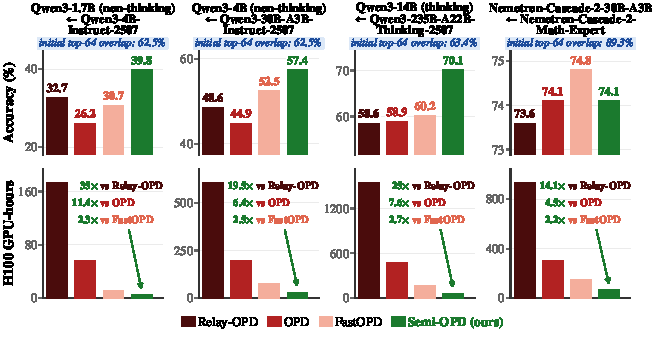
\includegraphics[width=0.95\linewidth]{figures/fig_teaser_speedup.pdf}
  \vspace{-0.5em}
\caption{
\textbf{Accuracy \& training cost of different distillation methods.} Our \method achieves much improved/comparable accuracy for teacher--student pairs with low/high overlap, respectively, while reducing training time by up to $11.4\times$ over OPD. 
Accuracy is averaged over AIME~24/25/26 and HMMT~Feb~26.
}
\label{fig:speedup}
  \endgroup
}

\makeatletter
\renewcommand{\maketitle}{%
  \twocolumn[%
    \begin{adjustwidth}{0pt}{24pt}%
      \begin{flushleft}%
        {\raggedright \titlefont \@title\par}%
        \vskip11pt%
        {\raggedright \@author\par}%
        \vskip20pt%
      \end{flushleft}%
    \end{adjustwidth}%
    \abscontent
    \vskip16pt
    \teaserfigure
    \vskip20pt%
  ]%
  \thispagestyle{firststyle}%
}
\makeatother


\begin{document}
\maketitle



\begin{figure*}[t]
  \centering
  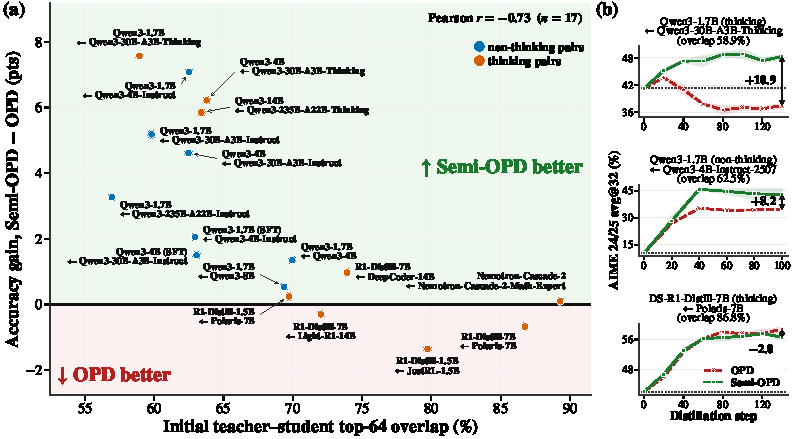
\includegraphics[width=0.95\linewidth]{figures/fig_overlap_combo.pdf}
  \vspace{-0.5em}
  \caption{
\textbf{当初始教师-学生重叠度较低时，Semi-OPD优于标准OPD。}
\textbf{(a)} 17对模型在从1.5B到235B规模范围内，涵盖思维模式与非思维模式以及多个模型家族的初始前64重叠度下的准确率提升情况，皮尔逊相关系数为$r=-0.73$。准确率提升是指Semi-OPD与OPD准确率曲线之间的面积差除以两者共享的训练周期，对AIME~24/25/26和HMMT~Feb~26取平均。
\textbf{(b)}~三个重叠度逐步增加的模型对的训练曲线（AIME~24/25平均@32，3个种子的均值）。在低重叠度下，Semi-OPD表现优于OPD，而OPD甚至可能出现性能下降；在高重叠度下，Semi-OPD可能略微落后。}
  \label{fig:overlap}
  \vspace{-1em}
\end{figure*}



\section{引言}
\label{sec:intro}

同策略蒸馏（OPD）已成为一种有效的方法，用于将教师语言模型（LM）的能力迁移至学生语言模型~\citep{agarwal2024policy, gu2024minillm, lu2025onpolicydistillation, xiao2026mimov2flashtechnicalreport, xu2026deepseek}。它通过在通过同策略采样获得的学生轨迹上提供来自教师语言模型的稠密 token 级信号，缓解了传统知识蒸馏中的训练-推理分布不匹配问题，即曝光偏差。 

尽管前景乐观，近期的研究揭示了同策略蒸馏（OPD）的若干缺陷：\citep{luo2026demystifying, yang2026eos, fu2026revisiting, yu2026mismatch} 发现同策略的滚动采样往往导致生成序列过长，并陷入自我修正环路，耗尽生成预算却无法输出结束符（EOS token）；\citep{zhang2026fast,ziheng2026less, liu2026prefix} 发现对学生滚动采样中后期 token 的监督通常无益，截断至短前缀即可满足需求；而 \citep{xu2026pass,jiang2026trajectory} 也发现，一旦学生模型确定了错误的推理方向，后续偏离方向的延续会产生不可靠的监督信号并浪费计算资源。这些缺陷引出了我们核心的问题：

\begin{center}
\vspace{-0.5em}
\emph{同策略采样对于任意教师-学生配对的蒸馏是否总是有益的？}
\vspace{-0.5em}
\end{center}



为回答这一问题，我们提出了一种简单且高效的替代方法——半同策略蒸馏（Semi-OPD），其中在任何训练开始前，仅从初始学生模型中采样一次轨迹，并在整个蒸馏过程中重复使用，从而使得轨迹生成和教师Logit生成均为离线进行。尽管轨迹来源固定，但目标与同策略蒸馏（OPD）相同，且学生模型的对数概率，因此每个token的优势值，会在每一步使用当前参数重新计算。

我们在17组教师-学生配对上进行了评估，涵盖15亿至2350亿参数的三种模型家族，在思考模式与非思考模式下均进行了测试，覆盖了OPD文献中最常用的师生配对。我们发现，Semi-OPD在其中14组上优于OPD，准确率最高提升达+13.6\%，训练速度最快提升11.4$\times$，如图~\ref{fig:speedup}所示；而在其余三组上，性能相当（差距在0.1\%--2.6\%之间）。  
这一现象促使我们进一步探究如何在Semi-OPD与OPD之间进行选择，以及为何Semi-OPD通常表现更优。


\noindent \textbf{如何在半监督同策略蒸馏（Semi-OPD）与同策略蒸馏（OPD）之间进行选择。}
我们发现，Semi-OPD相较于OPD的收益与初始教师模型和学生模型之间的对齐程度密切相关，这一对齐程度可通过输出token上的教师-学生前$k$名重叠比率来量化，如图~\ref{fig:overlap}a所示。
图~\ref{fig:overlap}b中的准确率演化曲线进一步表明：(1) 当该重叠比率较低时，持续从不断演化的学生模型中重新生成轨迹会使得训练逐渐偏离教师模型的轨迹，此时严格的同策略性反而适得其反；(2) 仅当教师模型与学生模型具有较高的重叠比率时，OPD才具有优势。 


\noindent \textbf{为什么同策略蒸馏（OPD）通常表现不如半同策略蒸馏（Semi-OPD）。} 我们的实证研究表明，有效的蒸馏需要在学生和教师两个方面都具备“同策略性”，前者可缓解曝光偏差，后者决定了蒸馏信号的有效性。OPD 改进了前者，但可能削弱了后者。

具体而言，对于对齐不充分的样本对，随着上下文长度的增长，OPD 生成的学生轨迹相对于教师会变得越来越异策略。这种问题无法通过简单的截断来解决，因为我们实证表明，覆盖不同推理阶段的监督信号至关重要。

相比之下，Semi-OPD 在初始学生轨迹上通常在较短的上下文中进行蒸馏，同时覆盖完整的轨迹，因此更加稳定。换句话说，Semi-OPD 以牺牲部分学生同策略性为代价，换取了更强的教师同策略性，这一点也与我们的观察一致：Semi-OPD 使学生接触到更多教师所偏好的 token。


我们旨在激发社区重新思考使用OPD的时机，并在有意义的情景下研究更强大的OPD变体。我们的工作主要收获总结如下：


\begin{itemize}[leftmargin=1.2em]
\vspace{-1em}
\item OPD仅在教师-学生对的输出token具有高重叠度时才有效；对于非对齐对，Semi-OPD在准确率和训练效率方面都是更好的选择。

\item 有效的蒸馏需要同时满足学生模型在训练轨迹上的同策略性以及与教师模型的接近性；而OPD更侧重前者，可能牺牲后者。

\item 鉴于目标领域和初始师生对，应根据测得的重叠比例来决定选择OPD还是半监督OPD，而不是盲目选择OPD。

\item 未来对OPD的研究应仔细选择师生配对，以确保实验情景具有意义。

\end{itemize}


\vspace{-0.5em}
\section{一种高效的同策略方法替代方案：半同策略蒸馏}
\vspace{-0.5em}

\label{sec:method}

\subsection{OPD的预备知识}

形式上，给定一个提示 $x \sim \mathcal{D}$，学生大模型 $\pi_\theta$ 会自回归地生成一个响应 $y=(y_1,\dots,y_T)$，访问前缀状态 $s_t=(x,y_{<t})$。其潜在的序列级目标是相对于固定教师 $\pi_T$ 的反向 $\mathrm{KL}(\pi_\theta(\cdot\mid x)\,\|\,\pi_T(\cdot\mid x))$。在实际操作中，一种常见的近似方法使用局部 token 级目标，仅在学生采样的 token 上评估教师-学生对数概率比，避免在每个位置进行全词表比较~\citep{lu2025onpolicydistillation, team2026kimi}。这得到了采样 token 目标：
\begin{equation}
\mathcal{L}_{OPD}(\theta)
=
\mathbb{E}_{x \sim \mathcal{D},\, y \sim \pi_\theta(\cdot \mid x)}
\left[
\sum_{t=1}^{T}
-A_t \cdot \log \pi_\theta(y_t \mid s_t)
\right],
\label{eq:opd}
\end{equation}
其中优势 $A_t
=
\log \pi_T(y_t \mid s_t)
-
\log \pi_\theta(y_t \mid s_t)$  在梯度中被视为常数。


如第~\ref{sec:intro} 节所述，近期工作已识别出同策略蒸馏（OPD）中的若干不良行为，例如重复的自我修正~\citep{luo2026demystifying,yang2026eos,fu2026revisiting}、对后续 token 的监督效果不佳~\citep{zhang2026fast,ziheng2026less}，以及一旦学生模型错误地确定方向后，监督变得不可靠~\citep{xu2026pass,jiang2026trajectory}。  
为研究蒸馏中同策略采样（on-policy sampling）的必要性，我们在第~\ref{sec:semi_opd_method} 节提出了一种简单替代方案——半同策略蒸馏（Semi-OPD）。




\begin{figure*}[t]
  \centering
  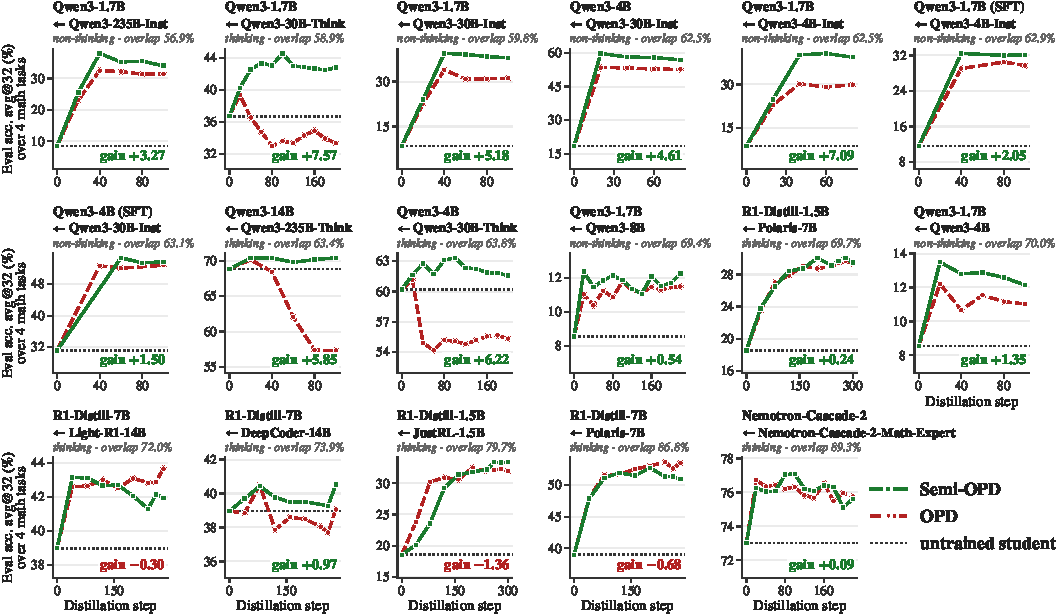
\includegraphics[width=0.95\linewidth]{fig3_allpairs.pdf}
\caption{
\textbf{半监督OPD与OPD在17组模型对中的对比。} 每个面板代表一组学生-教师模型对，其标题包含该对模型的初始前64重叠度。准确率以AIME 2024/2025/2026和HMMT 2026年2月的平均avg@32的均值衡量。每个面板中的数字是图~\ref{fig:overlap}a中绘制的增益，定义为两条曲线之间的面积除以训练周期。
  }
  \label{fig:allpairs}
  \vspace{-1em}
\end{figure*}




\subsection{半开放式配方}
\label{sec:semi_opd_method}

令 $\pi_0$ 表示初始学生，$\pi_\theta$ 表示正在被训练的学生。OPD 从当前学生 $y \sim \pi_\theta(\cdot \mid x)$ 中采样每个训练响应，因此训练数据会随着 $\theta$ 的更新而变化。半监督 OPD 则在训练开始前仅从初始学生中采样一次响应，
\begin{equation}
  \mathcal{D}_0 = \{(x_i, y_i)\}_{i=1}^{N}, \qquad y_i \sim \pi_0(\cdot \mid x_i).
\end{equation}
半OPD在整个训练过程中重复使用这个固定集合，以最小化与OPD相同的目標：
\begin{equation}
  \mathcal{L}_{\mathrm{\method}}(\theta)
  = \mathbb{E}_{(x,y) \sim \mathcal{D}_0}
  \Big[\sum_{t=1}^{T} -A_t \cdot \log \pi_\theta(y_t \mid s_t)\Big].
  \label{eq:semi-opd}
\end{equation}
尽管回溯轨迹是固定的，但学生模型的对数概率，以及由此产生的优势 $A_t$ ，是在每一步使用当前参数 $\theta$ 计算的，因此监督信号持续演化。



\noindent \textbf{Semi-OPD的训练效率。}
Semi-OPD将数据采集与最优化分离。我们首先从$\pi_0$生成所有学生轨迹；在这些响应生成后，仅需运行一次教师模型来计算教师的对数概率；最后，我们在固定的数据集和固定的教师对数概率上训练学生模型，无需进行任何在线轨迹生成或教师前向传播。此外，轨迹生成、教师评分和学生最优化作为独立阶段执行，每个阶段均可使用完整的GPU簇，而非在并发的学生生成、教师服务和训练之间划分资源。



\noindent \textbf{与 Lightning OPD 的比较。}  
先前的工作 Lightning OPD~\citep{wu2026lightning} 从一个基础学生模型出发，（1）在教师生成的轨迹上进行监督微调（SFT），（2）在离线的学生轨迹上进行蒸馏。由于它始终从一个无法生成高质量轨迹的基础模型开始，因此必须保留步骤（1）。而我们的 Semi-OPD 本质上省去了步骤（1），因为我们从指令微调过的学生模型出发，这更符合实际应用场景。我们在第~\ref{sec:experiments}/~\ref{sec:when_why} 节中表明，Semi-OPD 优于 Lightning OPD，且在教师轨迹上的 SFT 会产生负面影响。此外，我们利用该方法研究了 OPD 应在何时使用及其失败的潜在原因，为 OPD 的最佳实践提供了深入见解。

\vspace{-2mm}
\noindent \textbf{Top-$K$  重叠率，用于衡量初始教师-学生对齐程度。}
为衡量教师-学生对之间的对齐程度并覆盖实验中多样的组合情况，
我们遵循 \citep{li2026rethinking} 并比较初始学生回溯过程中每个响应位置上学生的和教师的
top-$K$  token 集合。具体而言，令   
$S_K(t) = \operatorname{TopK}(\pi_0(\cdot \mid s_t))$  和          
$T_K(t) = \operatorname{TopK}(\pi_T(\cdot \mid s_t))$  分别表示学生的   
和教师的 top-$K$  token 集合。我们将位置 $t$  处的 top-$K$  重叠率定义为
\[
\operatorname{Overlap@K}(t)
=
\frac{\left|S_K(t) \cap T_K(t)\right|}{K}.
\]
由于两组都包含 $K$ 个 token，当两个分布的前 $K$ 个支撑集相同时，该量为 $1$；当它们的支撑集互不重叠时，该量为 $0$。我们报告所有响应 token 的 token-权重平均值。除非另有说明，否则我们使用 $K=64$。


\begin{table*}[t]
\centering
\setlength{\tabcolsep}{7pt}
\renewcommand{\arraystretch}{0.85}
\caption{
当初始学生-教师重叠比率较低时，Semi-OPD优于其他OPD变体，而在比率较高时仍保持相当的性能。  
结果以温度为1.0时的avg@32报告，对60/80/100步的检查点进行平均。$^\S$ 来自~\citep{xu2026pass}。
}
\begin{tabular}{lccccc}
\toprule
Method
& AIME24 & AIME25 & AIME26 & HMMT Feb26 & Avg@32 \\
\midrule

\multicolumn{6}{l}{
\textbf{Qwen3-1.7B (Non-think) $\leftarrow$ Qwen3-4B-Instruct-2507 }
\hfill {\normalfont \underline{Initial overlap ratio: 62.5\%}}
} \\
\addlinespace[2pt]

\textit{Teacher}
& 60.4 & 46.0 & 52.2 & 31.2 & 47.5 \\
\textit{Student, untrained}
& 12.6 & 9.6 & 7.4 & 6.3 & 9.0 \\

\addlinespace[1pt]
Standard OPD$^\S$
& 35.8 & 25.5 & 23.3 & 20.1 & 26.2 \\
Speculative KD~\citep{xuspeculative}$^\S$
& 33.1 & 30.7 & 28.9 & 20.1 & 28.2 \\
FastOPD~\citep{zhang2026fast}$^\S$
& 42.3 & 30.4 & 26.4 & 23.6 & 30.7 \\
Lightning OPD~\citep{wu2026lightning}
& 41.0 & 28.8 & 27.5 & 22.7 & 30.0 \\
Relay-OPD~\citep{xu2026pass}$^\S$
& 42.7 & 32.8 & 30.5 & 24.7 & 32.7 \\
\textbf{\method (ours)}
& \textbf{50.3}
& \textbf{38.9}
& \textbf{41.8}
& \textbf{28.0}
& \textbf{39.8} \\


\midrule

\multicolumn{6}{l}{
\textbf{Qwen3-4B (Non-think) $\leftarrow$ Qwen3-30B-A3B-Instruct-2507}
\hfill {\normalfont \underline{Initial overlap ratio: 62.5\%}}
} \\
\addlinespace[2pt]

\textit{Teacher}
& 72.9 & 62.0 & 72.8 & 40.6 & 62.1 \\
\textit{Student, untrained}
& 23.6 & 18.0 & 16.8 & 14.9 & 18.3 \\

\addlinespace[1pt]
Standard OPD
& 55.1 & 45.3 & 49.1 & 30.0 & 44.9 \\
FastOPD~\citep{zhang2026fast}
& 63.5 & 55.5 & 56.2 & 34.9 & 52.5 \\
Lightning OPD~\citep{wu2026lightning}
& 64.0 & 56.8 & 54.3 & 33.5 & 52.2 \\
Relay-OPD~\citep{xu2026pass}
& 61.1 & 48.1 & 52.5 & 32.8 & 48.6 \\
\textbf{\method (ours)}
& \textbf{66.4}
& \textbf{63.1}
& \textbf{62.9}
& \textbf{37.4}
& \textbf{57.4} \\


\midrule







\multicolumn{6}{l}{
\textbf{NM-Cascade-2-30B-A3B $\leftarrow$ NM-Cascade-2-Math-Expert}
\hfill {\normalfont \underline{Initial overlap ratio: 89.3\%}}
} \\
\addlinespace[2pt]

\textit{Teacher}
& 82.8 & 80.0 & 76.4 & 58.2 & 74.4 \\
\textit{Student, untrained}
& 77.9 & 72.4 & 68.8 & 49.3 & 67.1 \\

\addlinespace[1pt]
Standard OPD
& 83.0 & 80.1 & 75.8 & 57.5 & 74.1 \\
FastOPD~\citep{zhang2026fast}
& 83.0 & \textbf{80.7} & \textbf{77.1} & \textbf{58.4} & \textbf{74.8} \\
Lightning OPD~\citep{wu2026lightning}
& \textbf{83.2} & 79.1 & 75.7 & 56.8 & 73.7 \\
Relay-OPD~\citep{xu2026pass}
& \textbf{83.2} & 80.1 & 73.3 & 57.7 & 73.6 \\
\textbf{\method (ours)}
& 83.0 & 79.7 & 77.0 & 56.8 & 74.1 \\

\bottomrule
\end{tabular}
\label{tab:baselines}
\vspace{-0.5em}
\end{table*}




\subsection{半OPD与OPD及其变体的基准测试}
\label{sec:experiments}
\vspace{-2mm}












\noindent \textbf{实验设置。}
我们在17组学生-教师模型对（完整的模型对名称见附录中的表~\ref{tab:allpairs}）上进行实验，涵盖Qwen3~\citep{qwen3}、DeepSeek-R1-Distill~\citep{deepseekai2025deepseekr1incentivizingreasoningcapability}和Nemotron-Cascade-2~\citep{yang2026nemotron}系列。Qwen3的学生模型（1.7B、4B和14B）从Instruct和Thinking教师模型中蒸馏而来，教师模型参数规模最高达235B-A22B，使用原始初始化或SFT预热初始化；DeepSeek-R1-Distill的学生模型（1.5B和7B）则从同一检查点的强化学习训练后代中蒸馏而来，包括JustRL~\citep{he2025justrl}、Polaris~\citep{Polaris2025}、Light-R1~\citep{lightr1proj}和DeepCoder~\citep{deepcoder2025}；而Nemotron-Cascade-2模型对由OPD步骤前的学生检查点及其用于OPD步骤的数学领域教师模型组成~\citep{yang2026nemotron}。这些模型对覆盖了非思考模式与思考模式，每组内的训练与评估均保持一致。所有模型均在DAPO-Math~\citep{yu2025dapo}上进行蒸馏。数学能力通过在AIME 2024--2026和HMMT February 2026上的$\mathrm{avg}@32$准确率来衡量，评估回放限制在32k token以内（Nemotron-Cascade-2为40k），跨领域泛化能力则在HumanEval和HumanEval+~\citep{chen2021evaluating}上评估。更多细节见附录~\ref{app:setup}。





\begin{figure*}[t]
  \centering
  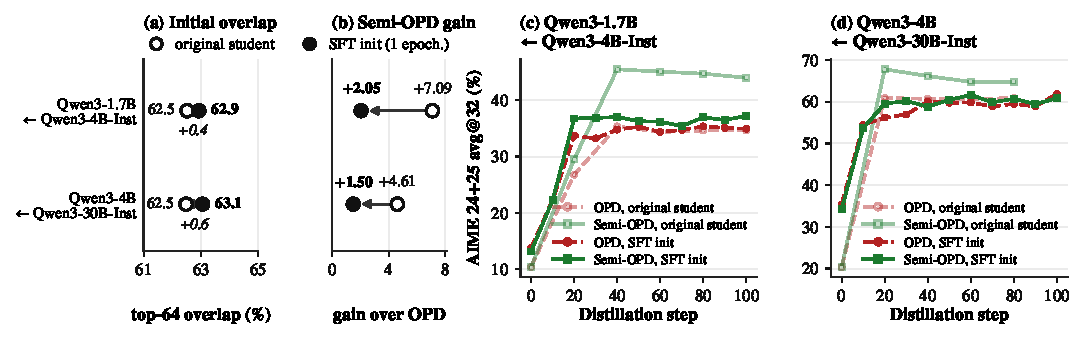
\includegraphics[width=\linewidth]{figures/fig_sft.pdf}
\vspace{-1.5em}
\caption{
\textbf{教师回放SFT提升了重叠率，但在半监督OPD后降低了最终性能。} \textbf{(a)} 在教师回放上进行SFT略微提高了初始的前64重叠率。 \textbf{(b)} 在教师回放上进行SFT后再进行半监督OPD，仍优于OPD，但表现不如仅使用半监督OPD。 \textbf{(c, d)} 在教师回放上进行SFT与半监督OPD结合后，对最终性能产生了负面影响。
}

  \label{fig:sft}
  \vspace{-1em}
\end{figure*}




\textbf{Semi-OPD 与 OPD 在 17 组模型对上的对比。} 图~\ref{fig:allpairs} 展示了在所有 17 组教师-学生模型对上，Semi-OPD 和 OPD 在训练过程中达到的平均准确率演化情况。我们按照初始教师-学生模型对的重叠比例对这些模型对进行排序，该比例标注在每个图表上方。此外，我们报告了 Semi-OPD 相对于 OPD 的平均准确率提升，其定义为 Semi-OPD 与 OPD 学习曲线之间的面积除以它们共享的训练周期。


我们观察到，在17对中的14对上，Semi-OPD的表现优于OPD，其在最后一步的提升最高可达$\sim$ 13\%，且在初始重叠度较低的配对上通常取得最大增益。在其余三对上，Semi-OPD仍能实现相当的性能，差距仅为0.1--2.6\%。对于Qwen3思考模式的配对，这种差异尤为明显：OPD在训练过程中出现显著的性能下降，而Semi-OPD则持续提升。




\noindent \textbf{与OPD变体在准确率和训练效率上的比较。} 除了标准OPD外，我们还针对三种不同模型大小、重叠比率和推理模式的模型对，将Semi-OPD与近期的OPD变体进行了对比，如表~\ref{tab:baselines}所示。我们观察到：(1) 在Qwen3-1.7B（非思考）和Qwen3-4B（非思考）学生模型上，其师生重叠比率较低，Semi-OPD在准确率方面优于所有其他基准方法，同时训练效率最高，例如，在这两个模型对上分别比Relay-OPD高出7.1\%和8.8\%的准确率，且训练时间分别减少了35$\times$和19.5$\times$，如图~\ref{fig:speedup}和表~\ref{tab:speedup}所示。(2) 在Nemotron-Cascade-2模型对上，其重叠比率约为89\%，我们的Semi-OPD仍与其他OPD基准方法保持竞争力，仅以0.7\%的准确率差距略逊于最佳基准，同时相比FastOPD将训练时间减少2.2倍，相比OPD减少4.5倍。

总体准确率-训练效率权衡如图~\ref{fig:speedup}所示，其中Semi-OPD相较于标准OPD实现了高达11.4$\times$的加速，相较于最快的基准方法FastOPD也实现了2.7$\times$的加速。相比之下，另一种OPD变体Relay-OPD虽然同样旨在使学生模型的生成更接近教师模型，但需要交替进行教师和学生的生成，导致效率较低。









\vspace{-0.5em}
\section{如何在门诊（OPD）与半门诊（Semi-OPD）之间进行选择？}
\vspace{-0.5em}
\label{sec:when_why}

如第~\ref{sec:experiments} 节和图~\ref{fig:allpairs} 所示，OPD 与 Semi-OPD 的相对性能与教师-学生重叠比例高度相关。因此，该指标可作为判断何时使用 OPD 或 Semi-OPD 的指示性依据。下文将更正式地描述这一相关系数。

\noindent \textbf{当教师-学生对的重叠比例较高时，需要使用OPD；否则，Semi-OPD更优且更快。} 我们在图~\ref{fig:overlap} 中计算了Semi-OPD相对于OPD的增益（以两者学习曲线之间的面积除以共享训练时段进行规范化的结果）与每对教师-学生重叠比例之间的相关系数。这两个量具有很强的相关性（17对中的皮尔逊相关系数为$r=-0.73$）：初始重叠比例较低的对从Semi-OPD中获益更大，而只有重叠比例较高的对才需要使用OPD。

该模式表明，当学生模型与教师模型存在显著差异时，反复从不断演化的学生策略中采样会导致在线回放质量下降（若干示例见附录~\ref{app:qualitative}），并削弱监督信号；而重用初始学生模型的回放数据可提供更稳定的蒸馏信号。我们将在第~\ref{sec:why} 节深入探讨其潜在原因。



\textbf{关键见解。}
上述现象为OPD的实际应用与研究提供了有益启示：(1) 针对特定的目标教师-学生对和目标领域提示，应根据其重叠比例来决定是否使用OPD或Semi-OPD，而非盲目采用OPD；(2) 未来在语言模型后训练流水线中研究改进的OPD方案时，需谨慎选择作为实验情景的教师-学生对；否则，Semi-OPD可作为强有力的基准。



\textbf{在教师生成的回放序列上进行SFT能否缩小差距？}
我们还进行了两组实验，其中学生模型在教师生成的回放序列上进行一轮SFT，随后进行OPD或半监督OPD。这与Lightning OPD~\citep{wu2026lightning}的设置一致。如图~\ref{fig:sft}所示，我们观察到：(1) 在教师回放序列上进行SFT略微提高了教师-学生重叠率，但半监督OPD在两组实验中仍优于OPD，尽管优势幅度较小；(2) 我们的半监督OPD在不包含额外的教师回放序列SFT阶段的情况下，性能反而优于包含该阶段的半监督OPD，表明在教师回放序列上进行SFT是不必要的。
此外我们注意到，尽管~\citep{wu2026lightning}将固定回放序列主要视为OPD的一种高效近似，但我们的结果表明，当初始教师-学生重叠率较低时，冻结回放缓存反而能提升蒸馏效果。



\begin{figure*}[t]
  \centering
  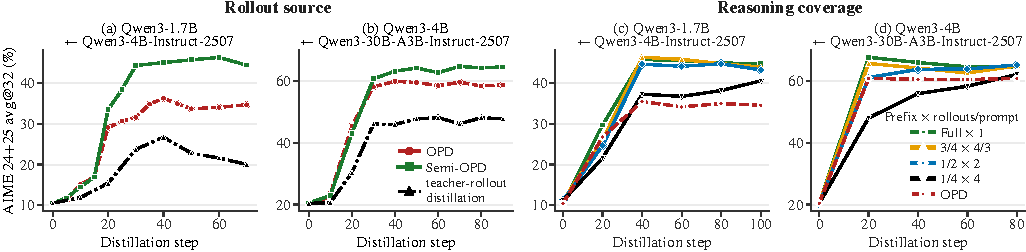
\includegraphics[width=\linewidth]{figures/fig_source_coverage.pdf}
  \vspace{-1em}
  \caption{
\textbf{rollout来源和推理覆盖对蒸馏都至关重要。}
\textbf{(a, b)} Semi-OPD在两组数据上均优于教师rollout蒸馏（以及OPD）。\textbf{(c, d)} 我们比较了在首个$1/4$、$1/2$、$3/4$或所有rollout阶段上训练的Semi-OPD，同时通过缩放每条提示的rollout数量来保持训练token总数不变。在所有阶段进行蒸馏的效果最佳。
}
  \label{fig:source_coverage}
  \label{fig:reasoning_coverage}
  \vspace{-0.5em}
\end{figure*}


\begin{figure}[t]
  \centering
  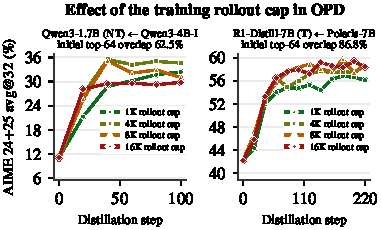
\includegraphics[width=\linewidth]{figures/fig_rollout_len.pdf}
  \vspace{-1.5em}
  \caption{
  更长的展开对重叠度低的一对（左）有负面影响，但对重叠度高的一对（右）没有影响。
  }
  \vspace{-1em}
  \label{fig:rollout_cap}
\end{figure}


\begin{figure*}[t]
  \centering
  \vspace{-0.5em}
  \begin{minipage}[t]{0.48\linewidth}
    \centering
    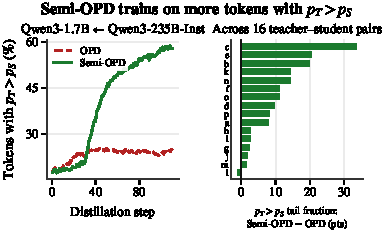
\includegraphics[width=\linewidth]{figures/fig_signal.pdf}
    \captionsetup{skip=4pt}
    \caption{\textbf{具有正奖励的token的百分比}，即在Semi-OPD和OPD下具有$p_T > p_S$的训练token的比例。}
    \label{fig:teacher_student_signal}
  \end{minipage}\hfill
  \begin{minipage}[t]{0.48\linewidth}
    \centering
    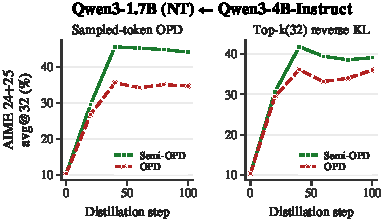
\includegraphics[width=\linewidth]{figures/fig_objective.pdf}
    \captionsetup{skip=4pt}
    \caption{\textbf{半监督OPD与OPD在两种蒸馏目标下的对比}，即，采样token和top-$k$ 逆KL目标。}
    \label{fig:distillation_objective}
  \end{minipage}
\end{figure*}


\begin{figure*}[t]
  \centering
  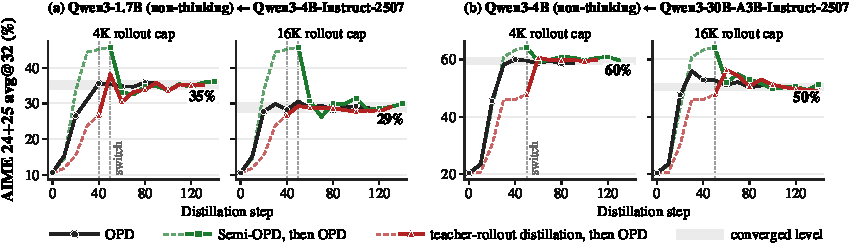
\includegraphics[width=\linewidth]{figures/fig_handoff.pdf}
    \vspace{-1.5em}
\caption{
\textbf{切换到OPD会趋向于一个由滚动预测决定的平衡状态，很大程度上与初始化无关。}
从初始学生模型、Semi-OPD检查点或教师滚动蒸馏检查点初始化时的OPD评估准确率轨迹。切换到OPD可能会降低或提升性能（见 \cref{fig:cache_switch_highoverlap}），其轨迹会趋近于在相同滚动上限下从头开始训练的OPD的性能水平。虚线表示切换到OPD之前的训练过程。
}
  \label{fig:handoff}
  \vspace{-1em}
\end{figure*}



\vspace{-0.5em}
\section{为什么OPD通常表现不如半透明OPD？}
\vspace{-0.5em}
\label{sec:why}

我们进一步探究了在重叠度较低的情况下，OPD性能不如Semi-OPD的原因。

\noindent \textbf{我们的假设。}
我们假设有效的蒸馏需要训练数据（即轨迹）满足两个特性：(1) 相对于学生模型的同策略性，以避免曝光偏差，以及 (2) 来自教师模型的高质量监督，这通常由相对于教师分布的同策略性决定，即轨迹与教师自身推理时分布的对齐程度。
同策略蒸馏（OPD）更注重前者，但在后者上表现不佳，尤其是在教师与学生之间重叠度较低的情况下；半同策略蒸馏（Semi-OPD）在一定程度上牺牲了学生模型的同策略性，以获得更有效的监督信号，如下文分析所示。

更具体地说，对于低重叠对，OPD 过程中的轨迹变得越来越长，并表现出各种伪影~\citep{luo2026demystifying, yang2026eos, fu2026revisiting}。这使得轨迹中较晚的 token 与教师的分布越来越偏离同策略，导致教师对这些 token 的监督变得无用甚至有害~\citep{xu2026pass,jiang2026trajectory}。  
截断轨迹并仅在前缀上进行训练可以缓解这一问题~\citep{zhang2026fast,ziheng2026less}，但代价是移除了对后期 token 的监督。如后续所示，在完整轨迹中覆盖所有推理阶段的监督信号对最终性能至关重要。  
相比之下，Semi-OPD 在初始学生生成的轨迹上进行训练，这些轨迹通常比同策略轨迹更短，从而在保持与教师分布的较好同策略性的同时，仍能覆盖包含所有推理阶段的完整轨迹。  
我们通过以下研究支持上述分析。


\noindent \textbf{学生同策略性的重要性：半同策略蒸馏与教师轨迹蒸馏对比。}
我们通过将初始学生轨迹缓存替换为教师生成的轨迹，同时保持其他所有情景不变，研究学生同策略性对半同策略蒸馏的影响。
如图~\ref{fig:source_coverage}(a, b)所示，半同策略蒸馏始终优于教师轨迹蒸馏。这表明半同策略蒸馏的优势并非仅仅来自于使用固定轨迹缓存。保留学生生成的轨迹以维持学生同策略性同样至关重要。




\noindent \textbf{在更长的回溯序列上进行训练可能会损害低重叠对的OPD表现。}  
如\cref{fig:rollout_cap}所示，我们调整了用于OPD训练的回溯序列长度（即回溯上限），观察到增加回溯上限会损害低重叠对的表现，而对高重叠对则有益。  
我们假设，对于低重叠对而言，在与教师策略异策略的长回溯序列上进行训练，可能倾向于强化表面化的推理模式，而未能充分改善潜在的推理过程，从而导致后续学生回溯序列的表现下降（回溯序列对比示例见附录~\ref{app:qualitative}）。


\noindent \textbf{覆盖所有推理阶段的监督信号至关重要。}  
如果长轨迹可能带来负面影响，一个简单的解决方案是截断它们，但这会损失后期推理阶段的监督信息。为隔离推理阶段覆盖的重要性，我们通过将缓存的半监督OPD迹（Semi-OPD traces）截断至其长度的前 $1/4$ 、$1/2$ 或 $3/4$ ，同时按比例调整每个提示的轨迹数量以保持总训练 token 预算不变，进行消融实验。如图~\ref{fig:reasoning_coverage}(c, d) 所示，仅保留前四分之一的监督会显著减慢收敛速度并降低最终准确率，而使用完整轨迹进行训练则达到最佳峰值准确率。因此，覆盖所有推理阶段以及保持与教师模型的同策略性均至关重要。




\noindent \textbf{Semi-OPD 使学生接触到更多教师偏好的 token。}  
Semi-OPD 通过较短的 rollout 长度实现完整轨迹覆盖，确切满足上述要求。为分析由此产生的蒸馏信号，我们测量训练过程中具有 $p_T > p_S$ 的 token 比例，即因教师赋予更高概率而获得正奖励的 token。  
如图~\ref{fig:teacher_student_signal} 所示，Semi-OPD 在整个训练过程中保持了比 OPD 更大比例的此类 token。这表明 Semi-OPD 使学生接触到更多教师偏好的 token，即相对于教师具有更高的同策略性，而 OPD 更常产生抑制学生自身采样 token 的信号。  
重要的是，如图~\ref{fig:distillation_objective} 所示，Semi-OPD 在 top-$k$ 反向 KL 下也优于 OPD，表明其优势并非仅针对采样 token 目标。


这些发现共同表明，半同策略动态（Semi-OPD）得益于保留对学生锚定的轨迹，这些轨迹能持续提供有效的教师监督，并广泛覆盖推理过程。在教师与学生模型差异较大的情况下，这些优势可超过完全同策略采样的好处。






































\vspace{-0.5em}
\section{更引人入胜的观察} 
\label{sec:training_dynamics}
\vspace{-0.5em}

除了主要对比之外，我们还观察到一些有趣的现象，这些现象有助于更全面地了解半开放式路径检测（Semi-OPD）与开放式路径检测（OPD）之间的差异。更多有趣的观察结果见附录。

\noindent \textbf{同策略蒸馏（OPD）会收敛到由回放轨迹决定的平衡点，与初始化无关。}
一个自然的问题是：在半同策略蒸馏（Semi-OPD）之后，OPD 是否还能进一步提升性能？我们通过从 Semi-OPD 或教师回放蒸馏检查点进行初始化作为热启动来研究这一问题。如图~\ref{fig:handoff} 所示，在低重叠对中，无论初始值如何，所有实验最终均收敛至在相同回放上限下从初始学生模型初始化的 OPD 所达到的性能水平，而热启动仅影响收敛轨迹。  
相比之下，在高重叠对中，如图~\ref{fig:cache_switch_highoverlap} 所示，从 Semi-OPD 切换到 OPD 能够提升性能，并弥合了大部分与从零开始应用 OPD 的差距。  
这表明重复的同策略采样推动蒸馏趋向于由在线回放数据分布决定的平衡点，而非初始检查点。对该平衡点的刻画仍是未来工作的一个有趣方向。


\begin{figure}[h]
  \centering
  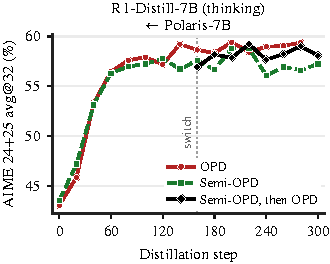
\includegraphics[width=0.8\linewidth]{figures/fig_cache_switch_polaris.pdf}
  \vspace{-0.5em}
  \caption{从半OPD切换到OPD，在重叠度较高的配对中，初始顶64重叠比为86.8\%时，可缩小与从头应用OPD的差距。}
  \label{fig:cache_switch_highoverlap}
\end{figure}


\noindent \textbf{收益会迁移到训练领域之外。}
如图~\ref{fig:code_transfer}所示，仅在数学密集型数据集~\citep{yu2025dapo}上蒸馏的模型在HumanEval和HumanEval+上也有所提升，且Semi-OPD仍然领先于OPD。
这表明这些收益并不局限于拟合数学训练分布，而是会迁移到更广泛的推理任务。


\begin{figure}[h]
  \centering
  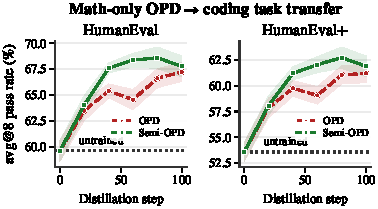
\includegraphics[width=\linewidth]{figures/fig_crossdomain.pdf}
  \vspace{-1.5em}
  \caption{\textbf{转换为代码。} 仅在数学上进行知识蒸馏的模型（Qwen3-1.7B $\leftarrow$  Qwen3-4B-Instruct-2507）的代码性能}
  \label{fig:code_transfer}
  \vspace{-1em}
\end{figure}

\begin{figure}[h]
  \centering
  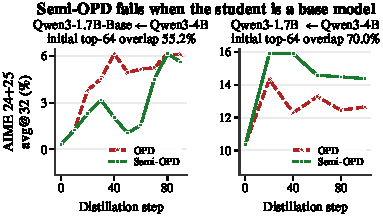
\includegraphics[width=\linewidth]{figures/fig_basestudent.pdf}
  \vspace{-1em}
   \caption{\textbf{初始学生能力。} 半OPD 与 OPD（相同教师），来自基础（左）和指令微调（右）的学生。}
    \label{fig:base_student}
    \vspace{-1em}
\end{figure}

\noindent \textbf{Semi-OPD 需要足够强的初始回溯轨迹。}  
由于 Semi-OPD 仅在来自 $\pi_0$ 的回溯轨迹上进行训练，因此初始回溯轨迹必须达到一定的质量阈值，才能实现有效的蒸馏。例如，如图~\ref{fig:base_student} 所示，使用基础学生模型时，初始回溯轨迹过于薄弱，导致 Semi-OPD 表现不如 OPD；而使用经过指令微调的学生模型时，Semi-OPD 重新展现出其优势。  
因此，当初始学生模型已能生成有意义的轨迹时，Semi-OPD 最为适用。
\vspace{-2mm}
\section{相关工作}
\vspace{-2mm}
\label{sec:related}

\textbf{同策略蒸馏及其机制。}
同策略蒸馏（OPD）在学生模型自身策略采样的轨迹上进行训练，而教师模型通过反向KL散度或相关目标提供稠密监督~\citep{agarwal2024policy,gu2024minillm,lu2025onpolicydistillation, song2026survey}。
通过优化学生自身访问分布的目标，OPD缓解了离线蒸馏中的曝光偏差问题~\citep{hinton2015distillingknowledgeneuralnetwork, kim2016sequence}，这一思想与交互式模仿学习方法（如DAgger）共享~\citep{ross2011reduction}。
近年来，OPD已成为推理模型后训练阶段的热门选择~\citep{xiao2026mimov2flashtechnicalreport,qwen3,xu2026deepseek,team2026kimi}，推动了近期研究对其中潜在机制的深入理解~\citep{jin2026entropy, fu2026revisiting, armandpour2026unmasking}。
例如，成功的OPD与教师-学生兼容性密切相关~\citep{li2026rethinking}，即使仅使用单个训练样本或1\%的token，也能恢复大部分全数据量下的OPD效果~\citep{fu2026rethinkingii, sheng20261}。

\textbf{OPD中的失败模式。}
近期工作识别出OPD的几种失败模式：学生模型的生成轨迹可能变长，陷入重复自我修正，并无法终止~\citep{luo2026demystifying,yang2026eos,fu2026revisiting,yu2026mismatch}，且生成轨迹的后半部分可能偏离教师模型的分布，导致监督信号日益不可靠~\citep{ziheng2026less,xu2026pass,jiang2026trajectory,wang2026demystifying}。
现有方法通过截断学生模型的生成轨迹~\citep{zhang2026fast,ziheng2026less}、在生成过程中让教师模型介入~\citep{xuspeculative,xu2026pass}、用教师模型优化学生轨迹~\citep{jiang2026trajectory}、在教师模型数据上对OPD进行预热~\citep{li2026rethinking}，或限制更新在信任区域以内~\citep{xing2026trust,xie2026trust}来缓解这些问题。
另有研究为提高效率而放松严格的同策略性，采用来自教师-SFT参考策略的固定生成轨迹~\citep{wu2026lightning,wu2026lightningii}，或在异步训练中使用策略滞后的学生生成轨迹~\citep{kang2026asyncopd}。
我们研究这种松弛的最简单形式：从初始学生模型中一次性采样生成轨迹，不经过任何教师-SFT阶段，也不进行刷新。
除了效率提升外，我们发现冻结生成轨迹还能提高准确率。
此外，不同于仅关注少数模型对，我们评估了17个多样化的模型对，并表明该优势与初始教师-学生前$k$名重叠度强相关，重叠度越低的模型对受益越多。




\vspace{-2mm}

\section{结论}
\vspace{-2mm}


本文重新审视了在语言模型蒸馏中同策略采样真正必要的情形。通过系统比较同策略蒸馏（OPD）与提出的半同策略蒸馏（Semi-OPD）在多种教师-学生组合上的表现，我们发现持续重新生成学生模型的轨迹通常并非必需，甚至在教师与学生对齐程度较差时可能造成负面影响。我们的分析揭示了一个关键原则：有效的蒸馏需要在学生和教师两个层面平衡同策略性，初始的教师-学生重叠度可作为判断何时采用OPD或Semi-OPD的实用指标。除了提供一种比OPD更高效的替代方案外，我们的研究还推动未来工作将同策略采样视为一种可选择的设计策略而非默认选项，并开发能够显式考虑教师-学生对齐程度与轨迹质量的蒸馏方法。






{
  \small
  \bibliographystyle{unsrt}
  \bibliography{ref}
}


\onecolumn
\appendix
\section{训练和评估设置}


\label{app:setup}

\paragraph{模型}
表~\ref{tab:allpairs} 列出了我们在实验中使用的全部17对教师-学生模型。它们涵盖了三个组别：  
(i)~Qwen3 学生（1.7B、4B、14B）从 Qwen3 Instruct-2507 与 Thinking-2507 教师模型中进行知识蒸馏，教师模型参数规模最高可达 235B-A22B；  
(ii)~DeepSeek-R1-Distill-Qwen 学生（1.5B、7B）从相同检查点的强化学习训练模型（JustRL、Polaris、Light-R1、DeepCoder）中进行蒸馏；  
(iii)~一个 Nemotron Cascade-2 数学专家对。  
对 (g) 和 (h) 在学生模型的 SFT 检查点基础上开始，随后在教师模型生成的回放数据上进行 1 轮次 SFT 训练。  
推理模式（思考模式 T / 非思考模式 NT）在每一对中固定且保持一致。同一对中的两种方法在训练和评估时均使用相同的聊天模板和推理模式，且评估模式始终与训练模式匹配。  
由于 DeepSeek-R1-Distill 的聊天模板始终预填充 \texttt{<think>}，因此我们将这些对视为思考模式。

\paragraph{训练数据和设置。}
所有实验均在来自 \href{https://huggingface.co/datasets/open-r1/DAPO-Math-17k-Processed}{DAPO-Math-17K dataset} 的提示上进行训练（去重后为 14{,}116 个英文提示），每步使用 128 个提示，每个提示生成一次采样。因此，一轮（Epoch）大约为 110 步。对于 Semi-OPD，我们在训练前从初始学生模型 $\pi_0$ 中对每个提示采样一个响应，采样参数和响应长度上限与 OPD 保持一致。OPD 按相同顺序读取提示。因此，两种方法在每一步看到的提示完全相同，仅在生成响应的模型上存在差异。两种方法均采用相同的采样 token 反向 KL 目标函数，且共享同一教师模型、学习率、批量大小和评估协议。表~\ref{tab:hparams} 列出了超参数。此外值得注意的是，在本工作中，Fast OPD 采用 4K 的训练采样回溯限制，遵循~\citep{xu2026pass}。对于仅非思考对的情况，我们在 \cref{fig:allpairs} 和 \cref{fig:overlap} 所示的对比中也对 OPD 采用 4K 的训练回溯长度。然而，在 \cref{tab:baselines} 中，为了与 Fast OPD 明确区分，OPD 对所有对均采用 16K 的回溯限制进行训练。关于训练期间使用的确切回溯形状，可参考 \cref{tab:allpairs}。需要注意的是，这是针对训练回溯长度，评估时我们均采用 32k 或 40k 的限制。

\begin{table}[h]
  \centering
  \small
  \caption{训练和评估超参数。 }
  \label{tab:hparams}
  \begin{tabular}{lcc}
    \toprule
    & Non-thinking pairs & Think/Long-CoT pairs \\
    \midrule
    \multicolumn{3}{l}{\emph{Optimization}} \\
    Optimizer & \multicolumn{2}{c}{AdamW ($\beta_1{=}0.9$, $\beta_2{=}0.999$, wd $0.01$)} \\
    Learning rate & \multicolumn{2}{c}{$1\times10^{-6}$, constant (no warm-up)} \\
    Gradient clipping & \multicolumn{2}{c}{1.0} \\
    Precision & \multicolumn{2}{c}{bfloat16} \\
    Prompts per step / rollouts per prompt & \multicolumn{2}{c}{128 / 1} \\
    Global batch size & \multicolumn{2}{c}{128} \\
    \midrule
    \multicolumn{3}{l}{\emph{Rollouts}} \\
    Max prompt length & \multicolumn{2}{c}{2{,}048} \\
    Max response length (training) & 4{,}096 & 16{,}384 \\
    Sampling temperature / top-$p$ & \multicolumn{2}{c}{1.0 / 1.0} \\
    \midrule
    \multicolumn{3}{l}{\emph{Loss}} \\
    Objective & \multicolumn{2}{c}{Sampled-token reverse KL} \\
    \midrule
    \multicolumn{3}{l}{\emph{Evaluation}} \\
    Benchmarks & \multicolumn{2}{c}{AIME24, AIME25, AIME26, HMMT Feb26} \\
    Metric & \multicolumn{2}{c}{avg@32} \\
    Temperature / top-$p$ & \multicolumn{2}{c}{1.0 / 1.0} \\
    Max response length & \multicolumn{2}{c}{32k (40k for Nemotron model)} \\
    \bottomrule
  \end{tabular}
\end{table}





\paragraph{基础设施。}
我们使用 NeMo-RL（DTensor 后端）进行训练，并使用 vLLM 生成滚动数据和评估样本。  
运行时根据教师模型的大小，使用 1–8 个结点，每个结点配备 8$\times$ \,H100 GPU。





\providecommand{\hf}[2]{\href{https://huggingface.co/#1}{#2}}
\begin{table}[h]
  \centering
  \small
  \caption{所有 17 组教师-学生对，按 Semi-OPD 相对于 OPD 的 AUC 增益排序。  
模型名称链接至使用的确切 Hugging Face 检查点。  
模式：T = 思维 / 长思维链，NT = 非思维。  
容量：训练回放的最大响应长度，Semi-OPD 与 OPD 共享。  
重叠：初始学生与教师之间的前 64 个 token 重叠百分比。  
最后一步：两种方法在最后一步评估时的 Semi-OPD 减去 OPD 差值。  
AUC：两种方法评估步骤范围内，两条准确率曲线之间的有符号面积，除以该跨度长度。  
增益为四个基准均值在 32 个点上的平均值。  
R1-Distill = DeepSeek-R1-Distill-Qwen；Cascade-2 = Nemotron-Cascade-2  
(SFT)：在教师回放上进行一轮 SFT 后的链接学生。  
$^\dagger$ 使用 40{,}960 token 的响应限制进行评估；其余所有组合均使用 32{,}768。}
  \label{tab:allpairs}
 \resizebox{\ifdim\width>\linewidth\linewidth\else\width\fi}{!}{%
  \begin{tabular}{cllccrrr}
    \toprule
    & & & & Train Len & Init. & \multicolumn{2}{c}{Gain} \\
    \cmidrule(lr){7-8}
    \# & Student & Teacher & Mode & Cap & Overlap & Last-step & AUC \\
    \midrule
    n & \hf{Qwen/Qwen3-1.7B}{Qwen3-1.7B} & \hf{Qwen/Qwen3-30B-A3B-Thinking-2507}{Qwen3-30B-A3B-Thinking} & T & 16K & 58.9 & \textbf{+9.4} & \textbf{+7.57} \\
    a & \hf{Qwen/Qwen3-1.7B}{Qwen3-1.7B} & \hf{Qwen/Qwen3-4B-Instruct-2507}{Qwen3-4B-Instruct-2507} & NT & 4K & 62.5 & \textbf{+9.5} & \textbf{+7.09} \\
    p & \hf{Qwen/Qwen3-4B}{Qwen3-4B} & \hf{Qwen/Qwen3-30B-A3B-Thinking-2507}{Qwen3-30B-A3B-Thinking} & T & 16K & 63.8 & \textbf{+6.2} & \textbf{+6.22} \\
    o & \hf{Qwen/Qwen3-14B}{Qwen3-14B} & \hf{Qwen/Qwen3-235B-A22B-Thinking-2507}{Qwen3-235B-A22B-Thinking} & T & 16K & 63.4 & \textbf{+13.1} & \textbf{+5.85} \\
    b & \hf{Qwen/Qwen3-1.7B}{Qwen3-1.7B} & \hf{Qwen/Qwen3-30B-A3B-Instruct-2507}{Qwen3-30B-A3B-Instruct-2507} & NT & 4K & 59.8 & \textbf{+6.8} & \textbf{+5.18} \\
    f & \hf{Qwen/Qwen3-4B}{Qwen3-4B} & \hf{Qwen/Qwen3-30B-A3B-Instruct-2507}{Qwen3-30B-A3B-Instruct-2507} & NT & 4K & 62.5 & \textbf{+4.2} & \textbf{+4.61} \\
    c & \hf{Qwen/Qwen3-1.7B}{Qwen3-1.7B} & \hf{Qwen/Qwen3-235B-A22B-Instruct-2507}{Qwen3-235B-A22B-Instruct-2507} & NT & 4K & 56.9 & \textbf{+2.6} & \textbf{+3.27} \\
    g & \hf{Qwen/Qwen3-1.7B}{Qwen3-1.7B} (SFT) & \hf{Qwen/Qwen3-4B-Instruct-2507}{Qwen3-4B-Instruct-2507} & NT & 4K & 62.9 & \textbf{+2.4} & \textbf{+2.05} \\
    h & \hf{Qwen/Qwen3-4B}{Qwen3-4B} (SFT) & \hf{Qwen/Qwen3-30B-A3B-Instruct-2507}{Qwen3-30B-A3B-Instruct-2507} & NT & 4K & 63.1 & +0.9 & +1.50 \\
    d & \hf{Qwen/Qwen3-1.7B}{Qwen3-1.7B} & \hf{Qwen/Qwen3-4B}{Qwen3-4B} & NT & 4K & 70.0 & +1.1 & +1.35 \\
    m & \hf{deepseek-ai/DeepSeek-R1-Distill-Qwen-7B}{R1-Distill-7B} & \hf{agentica-org/DeepCoder-14B-Preview}{DeepCoder-14B} & T & 16K & 73.9 & +1.5 & +0.97 \\
    e & \hf{Qwen/Qwen3-1.7B}{Qwen3-1.7B} & \hf{Qwen/Qwen3-8B}{Qwen3-8B} & NT & 4K & 69.4 & +0.8 & +0.54 \\
    j & \hf{deepseek-ai/DeepSeek-R1-Distill-Qwen-1.5B}{R1-Distill-1.5B} & \hf{POLARIS-Project/Polaris-7B-Preview}{Polaris-7B} & T & 16K & 69.7 & +0.1 & +0.24 \\
    q & Cascade-2-30B-A3B & Cascade-2-Math-Expert$^{\dagger}$ & T & 16K & 89.3 & $-$0.1 & +0.09 \\
    l & \hf{deepseek-ai/DeepSeek-R1-Distill-Qwen-7B}{R1-Distill-7B} & \hf{qihoo360/Light-R1-14B-DS}{Light-R1-14B} & T & 16K & 72.0 & $-$1.7 & $-$0.30 \\
    k & \hf{deepseek-ai/DeepSeek-R1-Distill-Qwen-7B}{R1-Distill-7B} & \hf{POLARIS-Project/Polaris-7B-Preview}{Polaris-7B} & T & 16K & 86.8 & $-$2.6 & $-$0.68 \\
    i & \hf{deepseek-ai/DeepSeek-R1-Distill-Qwen-1.5B}{R1-Distill-1.5B} & \hf{hbx/JustRL-DeepSeek-1.5B}{JustRL-1.5B} & T & 16K & 79.7 & +1.4 & $-$1.36 \\
    \bottomrule
  \end{tabular}}
\end{table}

\clearpage
\newpage

\section{所有配对间的训练动态}
\label{app:allpairs_dynamics}

我们在本节中提供更多训练动态讨论。\Cref{fig:allpairs_length,fig:allpairs_signal,fig:allpairs_student_entropy,fig:allpairs_teacher_entropy,fig:allpairs_overlap} 跟踪17对中16对（除Nemotron-级联-2对之外）的训练轨迹的五个属性。

\paragraph{展开长度。}
如\cref{fig:allpairs_length}所示，随着训练的进行，OPD的回溯序列长度逐渐增加，而Semi-OPD由于构造原因，其回溯序列长度始终保持在初始学生模型的回溯序列长度。在最后10个共享步骤中，16组中有15组的OPD回溯序列比Semi-OPD长7\%–113\%。对于重叠度低且不进行思考的Qwen3组合，这种增长最为显著，此时OPD的回溯序列长度常常超过教师模型自身的长度。唯一例外的是R1-Distill-1.5B $\leftarrow$ JustRL-1.5B，其OPD回溯序列反而变短。


\begin{figure}[H]
  \centering
  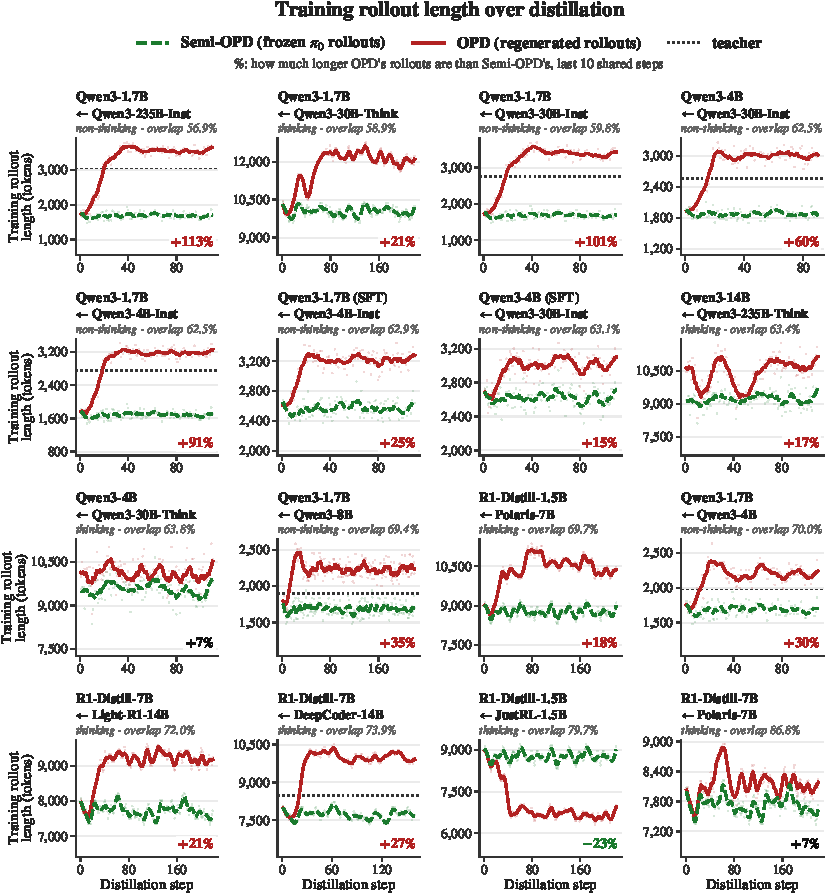
\includegraphics[width=0.85\linewidth]{figures/fig_allpairs_length.pdf}
  \caption{\textbf{训练展开长度。} 每次训练展开的平均生成 token 数。每个面板中的数字表示在最后 10 个共享步骤中，OPD 的展开比 Semi-OPD 长多少；虚线表示教师模型的展开长度（如可用）。}
  \label{fig:allpairs_length}
\end{figure}

\newpage
\paragraph{正向监督的token}
如\cref{fig:allpairs_signal}所示，半监督OPD在16组中的15组中保持了比OPD更多的正向监督token（$p_T > p_S$）。例外情况再次出现在R1-Distill-1.5B $\leftarrow$ JustRL-1.5B。



\begin{figure}[H]
  \centering
  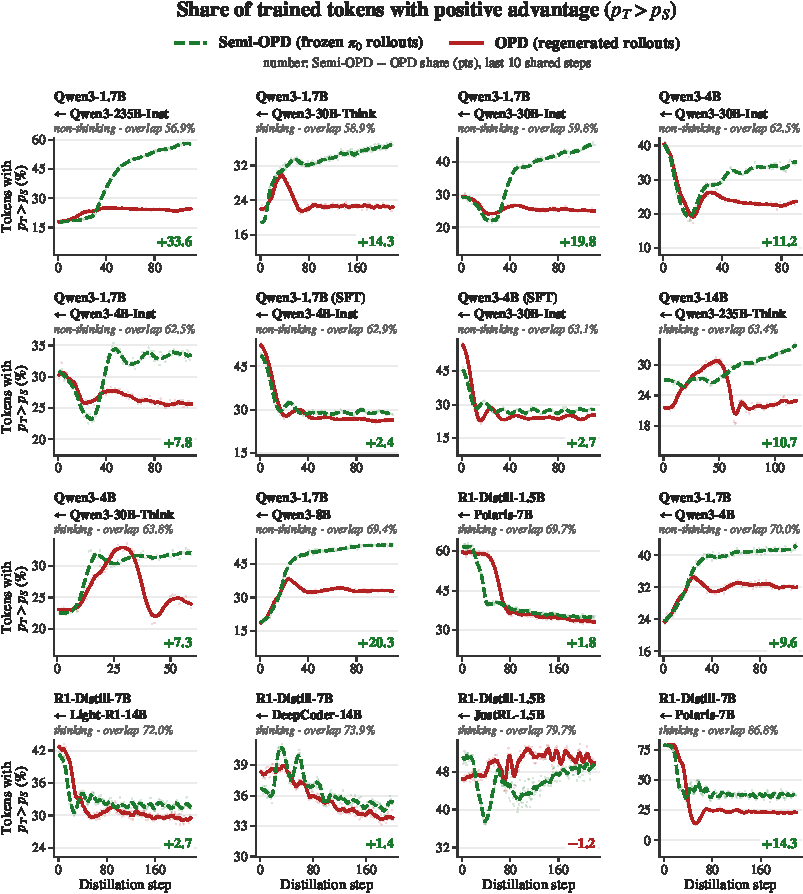
\includegraphics[width=0.85\linewidth]{figures/fig_allpairs_signal.pdf}
  \caption{\textbf{正向监督 token。} 与 $p_T > p_S$ 共享的训练 token 比例。每个面板中的数字为最后 10 个共享步骤中，Semi-OPD 减去 OPD 的差值，单位为点。}
  \label{fig:allpairs_signal}
\end{figure}

\clearpage
\newpage
\paragraph{学生与教师的熵。}
如\cref{fig:allpairs_student_entropy,fig:allpairs_teacher_entropy}所示，在思考配对中，OPD在8个配对中的7个（例外是R1-Distill-7B $\leftarrow$ DeepCoder-14B）将学生和教师的训练token上的下一token熵都推至远低于Semi-OPD的水平，即OPD越来越多地训练在两种模型均已高置信度预测的token上。在非思考配对中，两种方法下学生熵保持相似，而OPD下教师熵通常更高，表明OPD的rollout漂移到了教师不太确定的区域。

\begin{figure}[H]
  \centering
  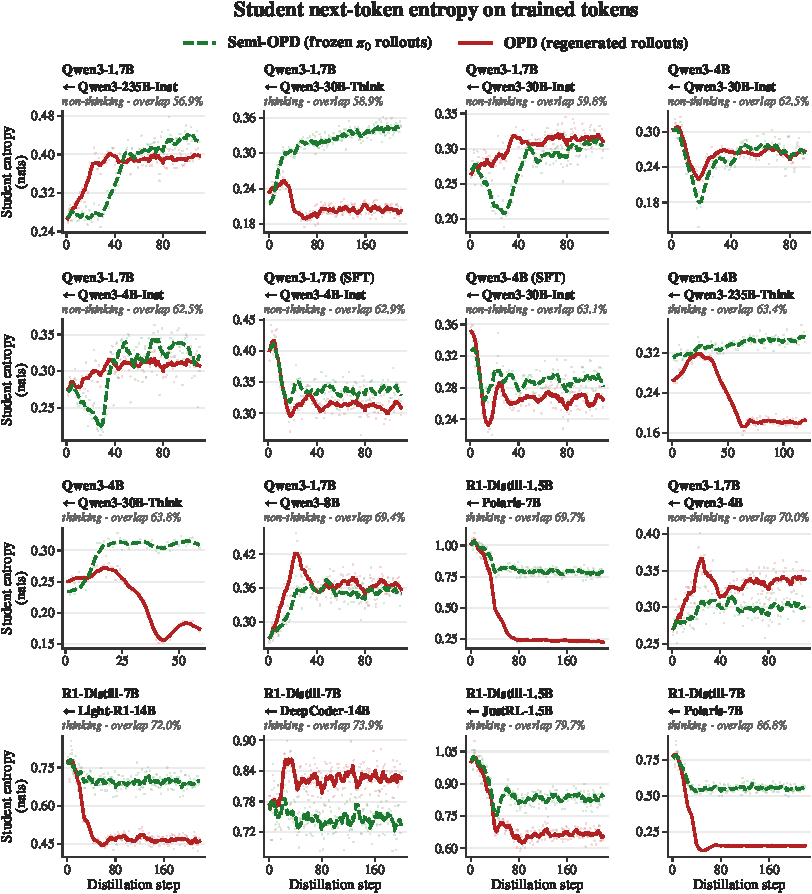
\includegraphics[width=0.85\linewidth]{figures/fig_allpairs_student_entropy.pdf}
  \caption{\textbf{学生熵。} 学生在训练 token 上的平均下一个 token 熵（nats）。}
  \label{fig:allpairs_student_entropy}
\end{figure}


\begin{figure}[H]
  \centering
  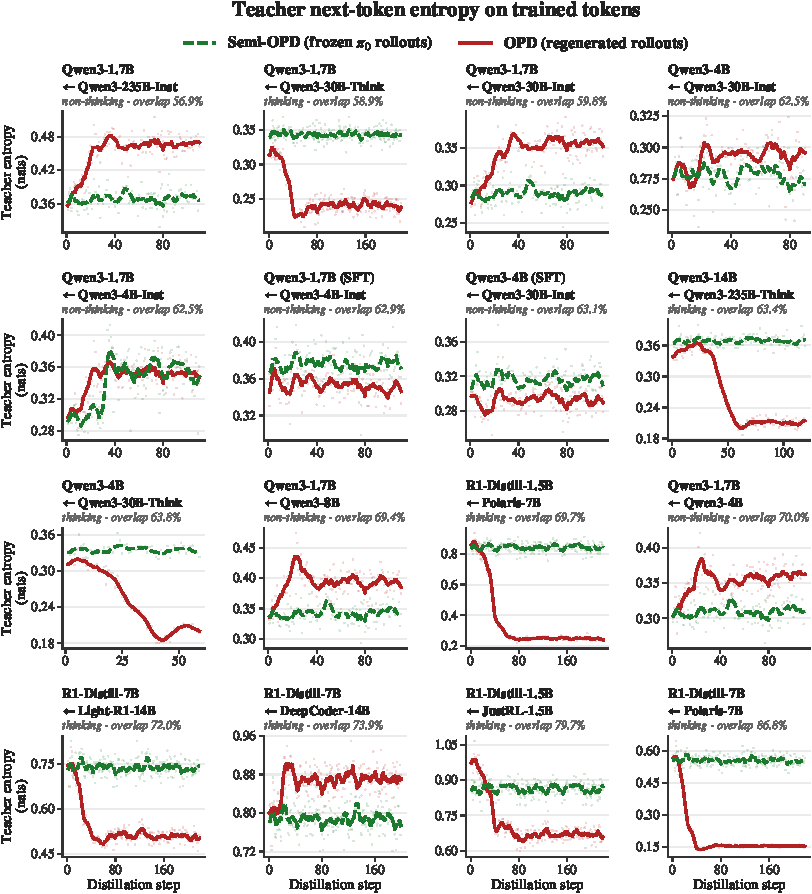
\includegraphics[width=0.85\linewidth]{figures/fig_allpairs_teacher_entropy.pdf}
  \caption{\textbf{教师熵。} 教师在相同训练 token 上的平均下一个 token 熵（nats），即教师在其监督的轨迹上有多不确定。}
  \label{fig:allpairs_teacher_entropy}
\end{figure}

\newpage
\paragraph{师生重叠。}
如图\cref{fig:allpairs_overlap}所示，在训练token上，随着学生模型向教师模型靠近，两种方法下当前学生与教师之间的前64个重叠通常都会增加，但不同模型对之间的排序存在差异。








\begin{figure}[H]
  \centering
  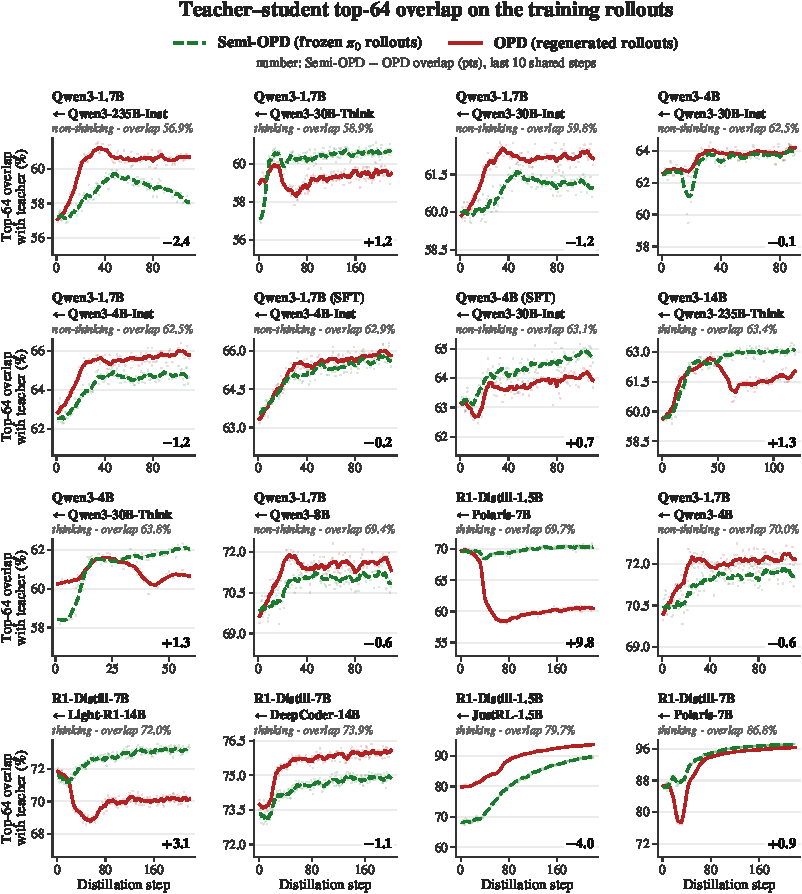
\includegraphics[width=0.85\linewidth]{figures/fig_allpairs_overlap.pdf}
  \caption{\textbf{教师与学生在训练轨迹上的重叠。} 当前学生与教师之间的前64个重叠项，基于每种方法自身的训练token计算，使用与\cref{sec:method}中初始重叠相同的度量标准。每个面板中的数字表示最后10个共享步骤中，Semi-OPD减去OPD的差值，单位为百分点。对于两个通过SFT初始化的配对，重叠仅在初始化和第110步时进行测量。}
  \label{fig:allpairs_overlap}
\end{figure}


\newpage

\section{训练成本对比}
Semi-OPD 更快，因为轨迹生成和教师评分在训练前仅需执行一次。与 Lightning OPD~\citep{wu2026lightning} 类似，这消除了训练环中的在线轨迹生成和教师推理，因此所有 GPU 都可用于轨迹生成、教师对数概率评分以及学生训练。对于固定的学⽣，相同的轨迹缓存也可在不同教师之间重复使用；评估新教师只需计算其在已缓存轨迹上的对数概率。这在实践中可进一步降低比较或选择教师的成本。相比之下，Relay-OPD 在整个训练过程中需要交替进行学生和教师的生成，导致更高的训练成本。

\begin{table*}[h]
  \centering
  \caption{\textbf{训练成本。} 100个训练步骤的H100 GPU小时数，不包括评估。
  Semi-OPD的成本是滚动生成、教师评分和学生训练之和。
  FastOPD是将滚动截断至4K token的OPD。加速比为该方法的GPU小时数除以Semi-OPD的GPU小时数。}
  \vspace{2mm}
  \label{tab:speedup}
  \setlength{\tabcolsep}{10pt}
  \renewcommand{\arraystretch}{1.15}
  \begin{tabular}{@{}lrr@{}}
    \toprule
    Method & GPU-hours & Semi-OPD speedup \\
    \midrule
    \multicolumn{3}{@{}l}{\textit{Qwen3-1.7B (non-thinking) $\leftarrow$ Qwen3-4B-Instruct-2507}$^{\dagger}$} \\
    \quad Relay-OPD & 173.3 & $34.7\times$ \\
    \quad OPD       & 56.8  & $11.4\times$ \\
    \quad FastOPD   & 11.7  & $2.3\times$ \\
    \quad \textbf{Semi-OPD} & \textbf{5.0} & -- \\
    \midrule
    \multicolumn{3}{@{}l}{\textit{Qwen3-4B (non-thinking) $\leftarrow$ Qwen3-30B-A3B-Instruct-2507}$^{\dagger}$} \\
    \quad Relay-OPD & 604.4 & $19.5\times$ \\
    \quad OPD       & 199.1 & $6.4\times$ \\
    \quad FastOPD   & 77.3  & $2.5\times$ \\
    \quad \textbf{Semi-OPD} & \textbf{31.0} & -- \\
    \midrule
    \multicolumn{3}{@{}l}{\textit{Qwen3-14B (thinking) $\leftarrow$ Qwen3-235B-A22B-Thinking-2507}} \\
    \quad Relay-OPD & 1546.5 & $24.6\times$ \\
    \quad OPD       & 480.0  & $7.6\times$ \\
    \quad FastOPD   & 169.8  & $2.7\times$ \\
    \quad \textbf{Semi-OPD} & \textbf{63.0} & -- \\
    \midrule
    \multicolumn{3}{@{}l}{\textit{Nemotron-Cascade-2-30B-A3B $\leftarrow$ Nemotron-Cascade-2-Math-Expert}} \\
    \quad Relay-OPD & 933.5 & $14.1\times$ \\
    \quad OPD       & 301.4 & $4.5\times$ \\
    \quad FastOPD   & 147.5 & $2.2\times$ \\
    \quad \textbf{Semi-OPD} & \textbf{66.4} & -- \\
    \bottomrule
  \end{tabular}\\[4pt]
  \begin{minipage}{0.85\linewidth}
  \footnotesize
  $^{\dagger}$ Semi-OPD 在这些数据对上使用 4K 训练滚动数据，而 OPD 使用 16K；在另外两组数据对上，两者均使用 16K。训练滚动数据上限列于 \cref{tab:allpairs}。\\
  \end{minipage}
\end{table*}


\clearpage
\newpage
\section{长度与自我修正膨胀}
\label{app:inflation}

图~\ref{fig:inflation} 跟踪了每种方法在训练过程中生成的轨迹的两个属性：轨迹长度（每个轨迹的平均生成 token 数）和自我修正词密度。在 OPD 情况下，当前学生会在每一步重新生成轨迹；在 Semi-OPD 情况下，这些轨迹是来自初始学生的冻结样本 $\pi_0$。

\paragraph{测量自我纠正能力。}
我们使用词汇密度来衡量自我修正。我们在生成的补全内容（不包括提示）中，统计一组固定自我修正词汇的不区分大小写、完整单词出现次数，即 \{\textit{wait, but, hmm, actually, hold, however, yet, oh, alternatively, no, ah, oops, well}\}。在每个训练步骤中，我们汇总全部 128 个训练回溯路径，并报告 $1000 \times \sum_i h_i / \sum_i c_i$ ，其中 $h_i$ 表示词频命中数，$c_i$ 表示回溯路径中的字符数，$i$ 为回溯路径编号。教师参考结果（虚线）在同一训练步骤最终提示上，对 128 个教师样本（$T{=}1.0$ ，相同的回溯路径上限）采用相同定义；教师的回溯长度也在相同样本上进行测量。由于词表包含 \textit{but} 和 \textit{no} 等常见话语词，该指标是反思性、犹豫式表达风格的代理度量，而非已验证修正次数的直接计数。我们在附录~\ref{app:qualitative} 中展示了 OPD 与 Semi-OPD 回溯路径对比的更多定性示例。

\begin{figure*}[h]
    \centering
    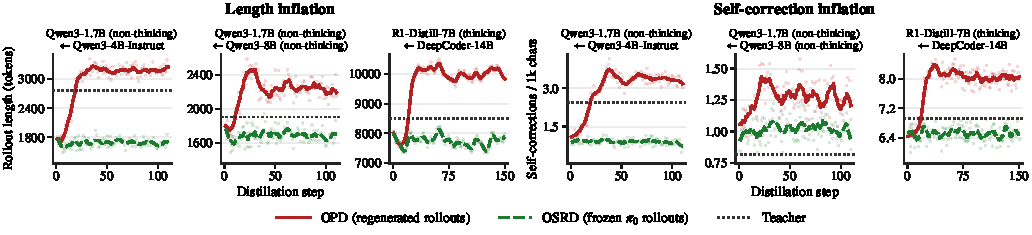
\includegraphics[width=\linewidth]{figures/fig_inflation.pdf}
    \caption{\textbf{同策略回溯在OPD期间被放大。}
    训练回溯的回溯长度（左侧三个面板）和自我修正词密度（右侧三个面板）。OPD回溯变得更长并使用更多的自我修正词，最终超过教师（虚线），而从初始学生 $\pi_0$ 一次性采样的冻结回溯则没有。}
    \label{fig:inflation}
\end{figure*}

\clearpage
\newpage
\section{定性示例：OPD 与半 OPD 训练部署}
\label{app:qualitative}



\providecommand{\refl}[1]{\textcolor{red}{\textbf{#1}}}
\providecommand{\capped}{{\color{gray}\textit{[generation cap reached; no final answer]}}}
\providecommand{\gap}[1]{{\color{gray}\textit{[\,\dots\ #1 tokens omitted\,\dots]}}}
\newtcolorbox{qualproblem}{colback=gray!6,colframe=gray!50,boxrule=0.4pt,arc=1pt,
  left=3pt,right=3pt,top=2pt,bottom=2pt,fontupper=\footnotesize}
\newtcolorbox{Semi-OPDbox}[1]{colback=white,colframe=green!45!black,boxrule=0.5pt,arc=1pt,
  left=2pt,right=2pt,top=1pt,bottom=1pt,toptitle=1pt,bottomtitle=1pt,
  fonttitle=\scriptsize\bfseries,fontupper=\scriptsize,title={#1},
  before upper={\setlength{\parskip}{2pt}\setlength{\parindent}{0pt}}}
\newtcolorbox{opdbox}[1]{colback=white,colframe=black!65,boxrule=0.5pt,arc=1pt,
  left=2pt,right=2pt,top=1pt,bottom=1pt,toptitle=1pt,bottomtitle=1pt,
  fonttitle=\scriptsize\bfseries,fontupper=\scriptsize,title={#1},
  before upper={\setlength{\parskip}{2pt}\setlength{\parindent}{0pt}}}



\begin{figure*}[h]
\centering
\begin{qualproblem}
\textbf{Example 1.} Qwen3-1.7B $\leftarrow$ Qwen3-30B-A3B-Thinking (thinking). OPD rollout at training step 201; Semi-OPD rollout from $\pi_0$; generation cap 16{,}384 tokens.\par\smallskip
\textbf{Problem.} What is the hundreds digit of the sum below?

$1 + 12 + 123 + 1234 + 12345 + 123456 + 1234567 + 12345678 + 123456789$
\end{qualproblem}
\vspace{-1pt}
\begin{minipage}[t]{0.495\linewidth}\vspace{0pt}
\begin{Semi-OPDbox}{Semi-OPD (frozen $\pi_0$ rollout): 5{,}688 tokens, 36 reflection words, reaches an answer}
\gap{1{,}101}

现在，对1000取模：205。

\refl{Wait}, so the total sum mod 1000 is 205? So the last three digits of the sum are 205. Therefore, the hundreds digit is 2. Is that correct?

\gap{2{,}535}

总计为137,174,205。

现在，最后三位数字是205，因此百位数字是2。这样就确认了。

\gap{1{,}380}

因此，和的百位数字是2。

\textbf{最终答案} \newline\rule{0pt}{2.6ex}$\boxed{2}$

\gap{550}
\end{Semi-OPDbox}
\end{minipage}\hfill
\begin{minipage}[t]{0.495\linewidth}\vspace{0pt}
\begin{opdbox}{OPD（步骤201）：16,384个token，80个反射词，达到上限}
\gap{6,594}

百位数字之和：0+0+1+2+3+4+5+6+7 = 28

加上十位的进位：28 + 4 = 32

和的百位数字：32 mod 10 = 2

\gap{2,658}

现在，和的百位是右边第二个数字，因此32 mod 100为32，所以百位数字是3

\gap{2,458}

\refl{啊}！这里有个错误：当我提到百位数字之和是28，加上十位的进位（4），这是百位的总和，即32。 \refl{但} 和的百位数字是32的个位数字，也就是2，而进位是3（进到千位）。

\gap{3,097}

\refl{等等}，不对。32是百位数字之和（加上进位）的结果，这表示百位的总值。例如，如果百位的和是32，意味着总和在百位上有3，在十位上有2？ \refl{不对}，数位的含义是：

- 如果百位的和是32，这意味着你有3×100 + 2×1，所以百位数字是3，十位数字是2。

\gap{1,140}

举个例子，如果百位数字之和加上进位是32，那么总值是32×100 +（余数），所以百位数字是2（即32的十位）。

\refl{等等}，不对：如果百位数字之和加上进位是32，那么百位对总和的贡献值是32×100。 \refl{但} 实际上，在加法中，百位是百位数，所以百位数字是总和中百位上的数字。

\capped
\end{opdbox}
\end{minipage}

\label{fig:qual_t1}
\end{figure*}







\begin{figure*}[p]
\centering
\begin{qualproblem}
\textbf{Example 2.} DeepSeek-R1-Distill-Qwen-7B $\leftarrow$ DeepCoder-14B (thinking). OPD rollout at training step 128; Semi-OPD rollout from $\pi_0$; generation cap 16{,}384 tokens.\par\smallskip
\textbf{Problem.} Find the positive solution to \newline $\frac 1{x^2-10x-29}+\frac1{x^2-10x-45}-\frac 2{x^2-10x-69}=0.$
\end{qualproblem}
\vspace{-1pt}
\begin{minipage}[t]{0.495\linewidth}\vspace{0pt}
\begin{Semi-OPDbox}{半开放问题解决框（冻结 $\pi_0$ 推演）：2{,}228 个 token，10 个反思词，得出答案}
\gap{176}

让我设 $y = x^2 - 10x$ 。于是，每个分母变为 $y - 29$ ，$y - 45$ ，和 $y - 69$ 。因此代入后，方程变为：

$\frac{1}{y - 29} + \frac{1}{y - 45} - \frac{2}{y - 69} = 0.$ 

\gap{769}

因此，方程简化为：

-64y +2496=0。

\gap{718}

\refl{但}题目要求正解，所以 x=13。

\gap{438}
\end{Semi-OPDbox}
\end{minipage}\hfill
\begin{minipage}[t]{0.495\linewidth}\vspace{0pt}
\begin{opdbox}{OPD（步骤128）：9{,}016个token，117个反射词，得出答案}
\gap{124}

我们设 $y = x^2 - 10x$ 。这似乎是一个聪明的置换，因为每个分母都可以用 y 表示。

\gap{1{,}916}

\refl{等等}，也许这是一个完全平方？让我检查一下257,664是否是平方数。

\refl{嗯}，508$^2$ =258,064。

507$^2$ =257,049。

相减得 257,664 -257,049=615。

不是完全平方。\refl{嗯}\dots{} \refl{等等}，也许615可以表示为……还不确定。

\gap{735}

\refl{等等}，也许最初的方法让我卡住了，因为平方根太复杂了。可能我之前计算有误？让我回头检查一下。

\refl{等等}，\refl{稍等}。让我重新梳理一下：

\gap{139}

\refl{等等}，\refl{稍等}，也许我在展开分母时出错了？

\refl{等等}，(y -29)(y -45)= y$^2$  -45y -29y +29$\times$ 45= y$^2$  -74y +1305？

\refl{等等}，29$\times$ 45：20$\times$ 45=900，9$\times$ 45=405，合计1305，这是正确的。

\refl{等等}，我之前交叉相乘时会不会犯了错误？让我再仔细核对一遍。

\gap{5{,}172}

因此，好的，逻辑成立。

步骤：代入 y=x$^2$  -10x，将方程化为仅含 y 的形式，解得 y=39，求得 x=13 和 x=-3，识别出所需解为正数。

因此，正解是13。

\gap{587}
\end{opdbox}
\end{minipage}

\label{fig:qual_ds7}
\end{figure*}


\begin{figure*}[p]
\centering
\begin{qualproblem}
\textbf{Example 3.} Qwen3-1.7B $\leftarrow$ Qwen3-30B-A3B-Instruct-2507 (non-thinking). OPD rollout at training step 90; Semi-OPD rollout from $\pi_0$; generation cap 4{,}096 tokens.\par\smallskip
\textbf{Problem.} Let $f(x) = \frac{x+1}{x-1}$. Then for $x^2 \neq 1$, find the expression for $f(-x)$. The original answer is in $\frac{k}{m}$ format, please give the value of $k + m$.
\end{qualproblem}
\vspace{-1pt}
\begin{minipage}[t]{0.495\linewidth}\vspace{0pt}
\begin{Semi-OPDbox}{半开放问题求解（冻结 $\pi_0$ 展开）：308 token，0 个反思词，得出答案}
\gap{69}

第 1 步：将 $-x$ 代入 $f(x)$

$f(-x) = \frac{(-x) + 1}{(-x) - 1}$

化简分子和分母：

$f(-x) = \frac{-x + 1}{-x - 1}$

我们可以从分子和分母中同时提出一个负号：

$f(-x) = \frac{-(x - 1)}{-(x + 1)} = \frac{x - 1}{x + 1}$

第 2 步：识别 $k$ 和 $m$

我们有：

$f(-x) = \frac{x - 1}{x + 1}$

这已经符合 $\frac{k}{m}$ 的形式，其中：

$k = -1,\allowbreak \quad m = 1$

第 3 步：计算 $k + m$

$k + m = -1 + 1 = \boxed{0}$

最终答案：

$\boxed{0}$
\end{Semi-OPDbox}
\end{minipage}\hfill
\begin{minipage}[t]{0.495\linewidth}\vspace{0pt}
\begin{opdbox}{OPD（步骤90）：4{,}096个token，87个反射词，达到上限}
\gap{239}

步骤3：检查其是否符合$\frac{k}{m}$的形式

这并非一个常数，而是一个关于$x$的有理函数，但我们需假设其形式为$\frac{k}{m}$，即一个常数。\refl{等等}——也许我们理解错了？

\gap{156}

\refl{等等}——但$f(-x)$并不是一个常数函数。只有当$x$是常数时才成立——但$x$是一个变量。

除非——也许题目是个陷阱？

\refl{等等}——让我们重新核对一下。

\gap{151}

\refl{等等}——也许题目并非要求$f(-x)$，而是要求将$f(-x)$的表达式化简为一个常数形式？

\refl{等等}——但$f(-x) = \frac{x - 1}{x + 1}$并不恒为常数。

\gap{510}

\refl{等等}——\textbf{也许原题存在笔误？}

\gap{531}

\refl{等等}——继续推进。

\refl{等等}——\textbf{假设原始答案是$\frac{1}{2}$}

\gap{466}

\refl{等等}——\textbf{终于！} 假设题目表述有误。

\gap{1{,}658}

\refl{等等}——也许原本应该是求$f(-x)$在特定$x$处的\textbf{值}？\refl{但}不是。

\refl{等等}——也许题目是在要求用$f(x)$表示$f(-x)$的表达式？

\gap{100}

\capped
\end{opdbox}
\end{minipage}

\label{fig:qual_q30i}
\end{figure*}

\FloatBarrier









\end{document}
